\documentclass[runningheads]{llncs}

\usepackage[T1]{fontenc}
\usepackage{graphicx}
\usepackage{booktabs}
\usepackage{multirow}
\usepackage{cite}
\usepackage{float}

\begin{document}
\sloppy
\title{Pseudo-MOS Learning: A Full-to-No-Reference FIQA Framework}

\author{André Neto\inst{1,2}\orcidID{0009-0001-0398-5859} \and % chktex 8
Nuno Gonçalves\inst{1,2}\orcidID{0000-0002-1018-4945}} % chktex 8
%
\authorrunning{A. Neto and N. Gonçalves}
% First names are abbreviated in the running head.
% If there are more than two authors, 'et al.' is used.

\institute{University of Coimbra, Portugal \and
Institute of Systems and Robotics, Coimbra, Portugal \\
\email{andre.neto@isr.uc.pt, nunogon@deec.uc.pt}}

\maketitle% typeset the header of the contribution

\begin{abstract}
This paper examines the correlation between 41 objective Image Quality Assessment (IQA) metrics and Mean Opinion Scores (MOS) across 102 facial images, each modified using four steganography methods at nine encoding levels. As IQA metrics are widely used to approximate human perception, understanding their reliability in the context of facial image distortion is crucial for applications in biometrics, forensics, and secure communication.  Using Pearson's and Spearman's correlation coefficients, we rank IQA metrics and evaluate fusion approaches, including PCA, regression, and machine learning. Our analysis also explores demographic (age, gender, ethnicity) and non-demographic (attractiveness) biases in MOS, highlighting significant perceptual variations across observer and subject groups.

\end{abstract}

\begin{IEEEkeywords}
FIQA, IQA, MOS, steganography, demographic bias, non-demographic bias, fusion techniques.
\end{IEEEkeywords}
\section{Introduction}

Image Quality Assessment (IQA) plays a critical role in domains such as biometric authentication, multimedia processing, and medical imaging~\cite{kim2015face, huang2020facerecon}. It broadly refers to the estimation of visual quality based on attributes like contrast, sharpness, noise, and the presence of artifacts. Within this domain, Facial Image Quality Assessment (FIQA) focuses specifically on facial images, where quality is not assessed in terms of visual aesthetics, but rather in terms of its impact on the performance of face recognition systems~\cite{cavazos2021racebias, terhoerst2020demobias}.

IQA methods fall into two categories: subjective and objective. Subjective methods use human ratings to measure perceived quality, often summarized as Mean Opinion Scores (MOS)~\cite{ITU-R-BT500}. These scores are reliable but expensive to collect and not scalable. Objective methods rely on algorithms to estimate quality, either by comparing to a reference image or by analyzing features of the image itself.

Objective methods can be divided into full-reference (FR) and no-reference (NR). FR methods compare a distorted image to a clean reference. They are often accurate but can only be used when a reference is available. NR methods estimate quality without a reference and are more practical in real-world settings, though they often struggle to generalize across distortions and content~\cite{shahrukh2019survey}.

FIQA is a subdomain of IQA focused on facial images. It plays a key role in biometric applications such as identity verification, where reference images are typically unavailable, and is also relevant in non-biometric scenarios like surveillance and forensic analysis. Consequently, most FIQA methods are no-reference NR, relying on task-specific priors or learned representations to estimate image quality~\cite{hernandez2019faceqnet}.

A key challenge in IQA is the gap between objective metrics and human perception. Classical metrics such as PSNR~\cite{gonzalez2002digital} (Peak Signal-to-Noise Ratio), SSIM~\cite{wang2004ssim} (Structural Similarity Index), and VIF~\cite{sheikh2006image} (Visual Information Fidelity) provide automatic quality estimates but often show weak correlation with human ratings across datasets~\cite{shahrukh2019survey}. This issue is more pronounced in facial images, where perceived quality is shaped by both image distortions and biases from the observer.

Studies have shown that FIQA is affected by both demographic and non-demographic biases. Perceived quality can vary with ethnicity, gender, or age, often due to dataset imbalance and observer subjectivity~\cite{cavazos2021racebias, terhoerst2020demobias, kabbani2024demo}. For example, darker skin tones tend to produce lower recognition accuracy, and female faces are often rated with lower quality scores~\cite{huang2020facerecon}. These effects highlight the need for more inclusive and perceptually aligned quality metrics.

The International Civil Aviation Organization~\cite{icao-2015} (ICAO) and the International Organization for Standardization (ISO) and the International Electrotechnical Commission (IEC) 19794--5 standard~\cite{iso-iec29794-5-2010} establish guidelines for image quality in Machine-Readable Travel Documents (MRTDs). These guidelines ensure uniform image conditions (e.g., lighting, focus, and resolution) and consistency across datasets. While these regulations establish a technical baseline, they do not account for perceptual biases and demographic variability in FIQA.\@

These biases raise ethical concerns. Legal frameworks, such as the European Convention on Human Rights (Article 14)~\cite{echr-article14}, the Universal Declaration of Human Rights (Article 7)~\cite{udhr-article7}, the General Data Protection Regulation (Article 22)~\cite{gdpr-article22}, the European Artificial Intelligence Act (2024)~\cite{eu-ai-act-2024} and the United States Bill of Rights~\cite{us-ai-bill-rights-2022}, aim to prevent discriminatory decisions. Still, biases persist, often introduced through human observers involved in labeling.

Neuroscience shows that face perception relies on the fusiform face area, a brain region specialized for facial stimuli~\cite{kanwisher2006fusiform, tsao2008mechanisms}. This biological specialization makes FIQA particularly sensitive to both stimulus features (e.g., age, gender, ethnicity, attractiveness) and the demographic background of the observers.

Steganographically distorted facial images pose a harder problem. Steganography hides data by slightly changing pixel values, often in ways that escape human detection~\cite{steganography}. Recent printed-proof techniques go further by ensuring that hidden data can survive physical printing and scanning noises, making them useful for secure document encoding. While these changes are visually minimal, they can damage biometric features and reduce recognition accuracy~\cite{stegastamp2020, codeface2021, stampone2024, riemannian2023}. NR methods are usually not designed to catch these small but critical degradations.

To handle these limitations, we propose a FIQA framework based on pseudo-MOS.\@ We first use a small set of facial images labeled with overall quality scores to train a fusion model that combines FR metrics into a single predictor. This model generates pseudo-MOS for the rest of the dataset. Using these labels, we then train a NR deep regressor based on a ResNet-18~\cite{resnet} pretrained on ImageNet~\cite{imagenet}, allowing it to estimate perceptual quality without needing a reference image.

Our approach bridges the gap between FR supervision and NR inference. It offers a scalable solution for evaluating images with subtle distortions, like steganography, and supports the development of quality assessment models tailored to domain-specific tasks. In doing so, it combines the accuracy of FR metrics with the practicality of NR models in a single IQA pipeline.

\section{Related Work}

Several fusion-based approaches have been proposed to better align IQA metrics with human perception. Liu et al.~\cite{liu2013mmf} introduced a multi-method fusion framework in which multiple FR-IQA scores are linearly combined through regression to better approximate human judgments. Similarly, Henniger et al.~\cite{henniger2020biosig} developed a Random Forest model trained on handcrafted image features drawn from ISO face quality standards, improving predictive utility for biometric applications. These works show that fusing complementary quality cues improves correlation with MOS compared to single-metric methods

In the absence of subjective labels, several methods have adopted weakly supervised strategies based on pseudo-labels. Chen et al.~\cite{chen2021pseudo} generated pseudo-MOS scores by averaging multiple FR-IQA scores. RankIQA~\cite{liu2017rankiqa} used synthetic degradations and ranking-based supervision to learn ordinal quality relationships. Wu et al.~\cite{wu2020cnn} trained cascaded CNN regressors on pseudo-MOS to support NR-IQA training. These methods show that pseudo-labeling can guide deep quality models when ground-truth MOS is limited.

Recent NR-IQA methods leverage deep features from CNNs pretrained on large datasets. Kang et al.\cite{kang2014cnn} showed that CNNs can directly predict image quality from patches. In FIQA, SER-FIQ\cite{terhorst2020serfiq} (Stochastic Embedding Robustness for Face Image Quality) estimates quality by measuring the consistency of face embeddings under dropout. MagFace~\cite{meng2021magface} links embedding magnitude to recognition performance to learn quality-aware features. FaceQnet~\cite{hernandez2019faceqnet} estimates how well a face image will perform in recognition tasks, using a regression model trained on features from a pre-trained network. QualFace~\cite{tremoco2021qualface} adapts face recognition networks for document images and adds a quality estimation branch aligned with ICAO and ISO/IEC standards. These approaches replace handcrafted indicators with learned representations optimized for face recognition.

Other studies emphasize that image quality is inherently task-specific. In FIQA, quality is defined not by visual aesthetics but by its effect on recognition performance. Standards such as ISO/IEC 19794--5 codify this operational perspective, specifying conditions for acceptable biometric image acquisition. Datasets such as PIPAL~\cite{pipal} and TID2013~\cite{tid2013}, which include generative distortions, further highlight the need for context-specific IQA evaluation. Our work follows this trajectory by targeting steganographically degraded facial images, an emerging use case not addressed in current FIQA literature.

\section{Methodology}\label{sec:methodology}

\subsection{Dataset}

Our dataset is derived from the publically available Face Research Lab London~\cite{frll} (FRLL) set, comprising 102 frontal ICAO-compliant facial images. Each image was encoded using four printer-proof steganographic methods, described ahead, each applied at nine different intensity levels, yielding a total of 3,672 distorted images.

The dataset was partitioned into four subsets, as follows:

\begin{itemize}
    \item MOS set (15 identities, 540 images): a core set of demographically diverse subjects, shown in Fig.~\ref{fig:mos_set}, with subjective MOS annotations. It is split into:
    \begin{itemize}
        \item MOS train set (12 identities): used to train the FR fusion model, regressing FR-IQA metrics to human MOS.\@
        \item MOS test set (3 identities): held out from the framework and used only for final evaluation.
    \end{itemize}
    \item Pseudo-MOS set (87 identities, 3,132 images): no subjective scores were collected for these images. Pseudo-MOS are generated for this set using the trained fusion model.
    \item NR train set: includes both the MOS train set and the pseudo-MOS set. It is used to train the NR regressor.
\end{itemize}

\begin{figure}
    \centering
    \begin{minipage}[t]{0.76\textwidth}
        \centering
        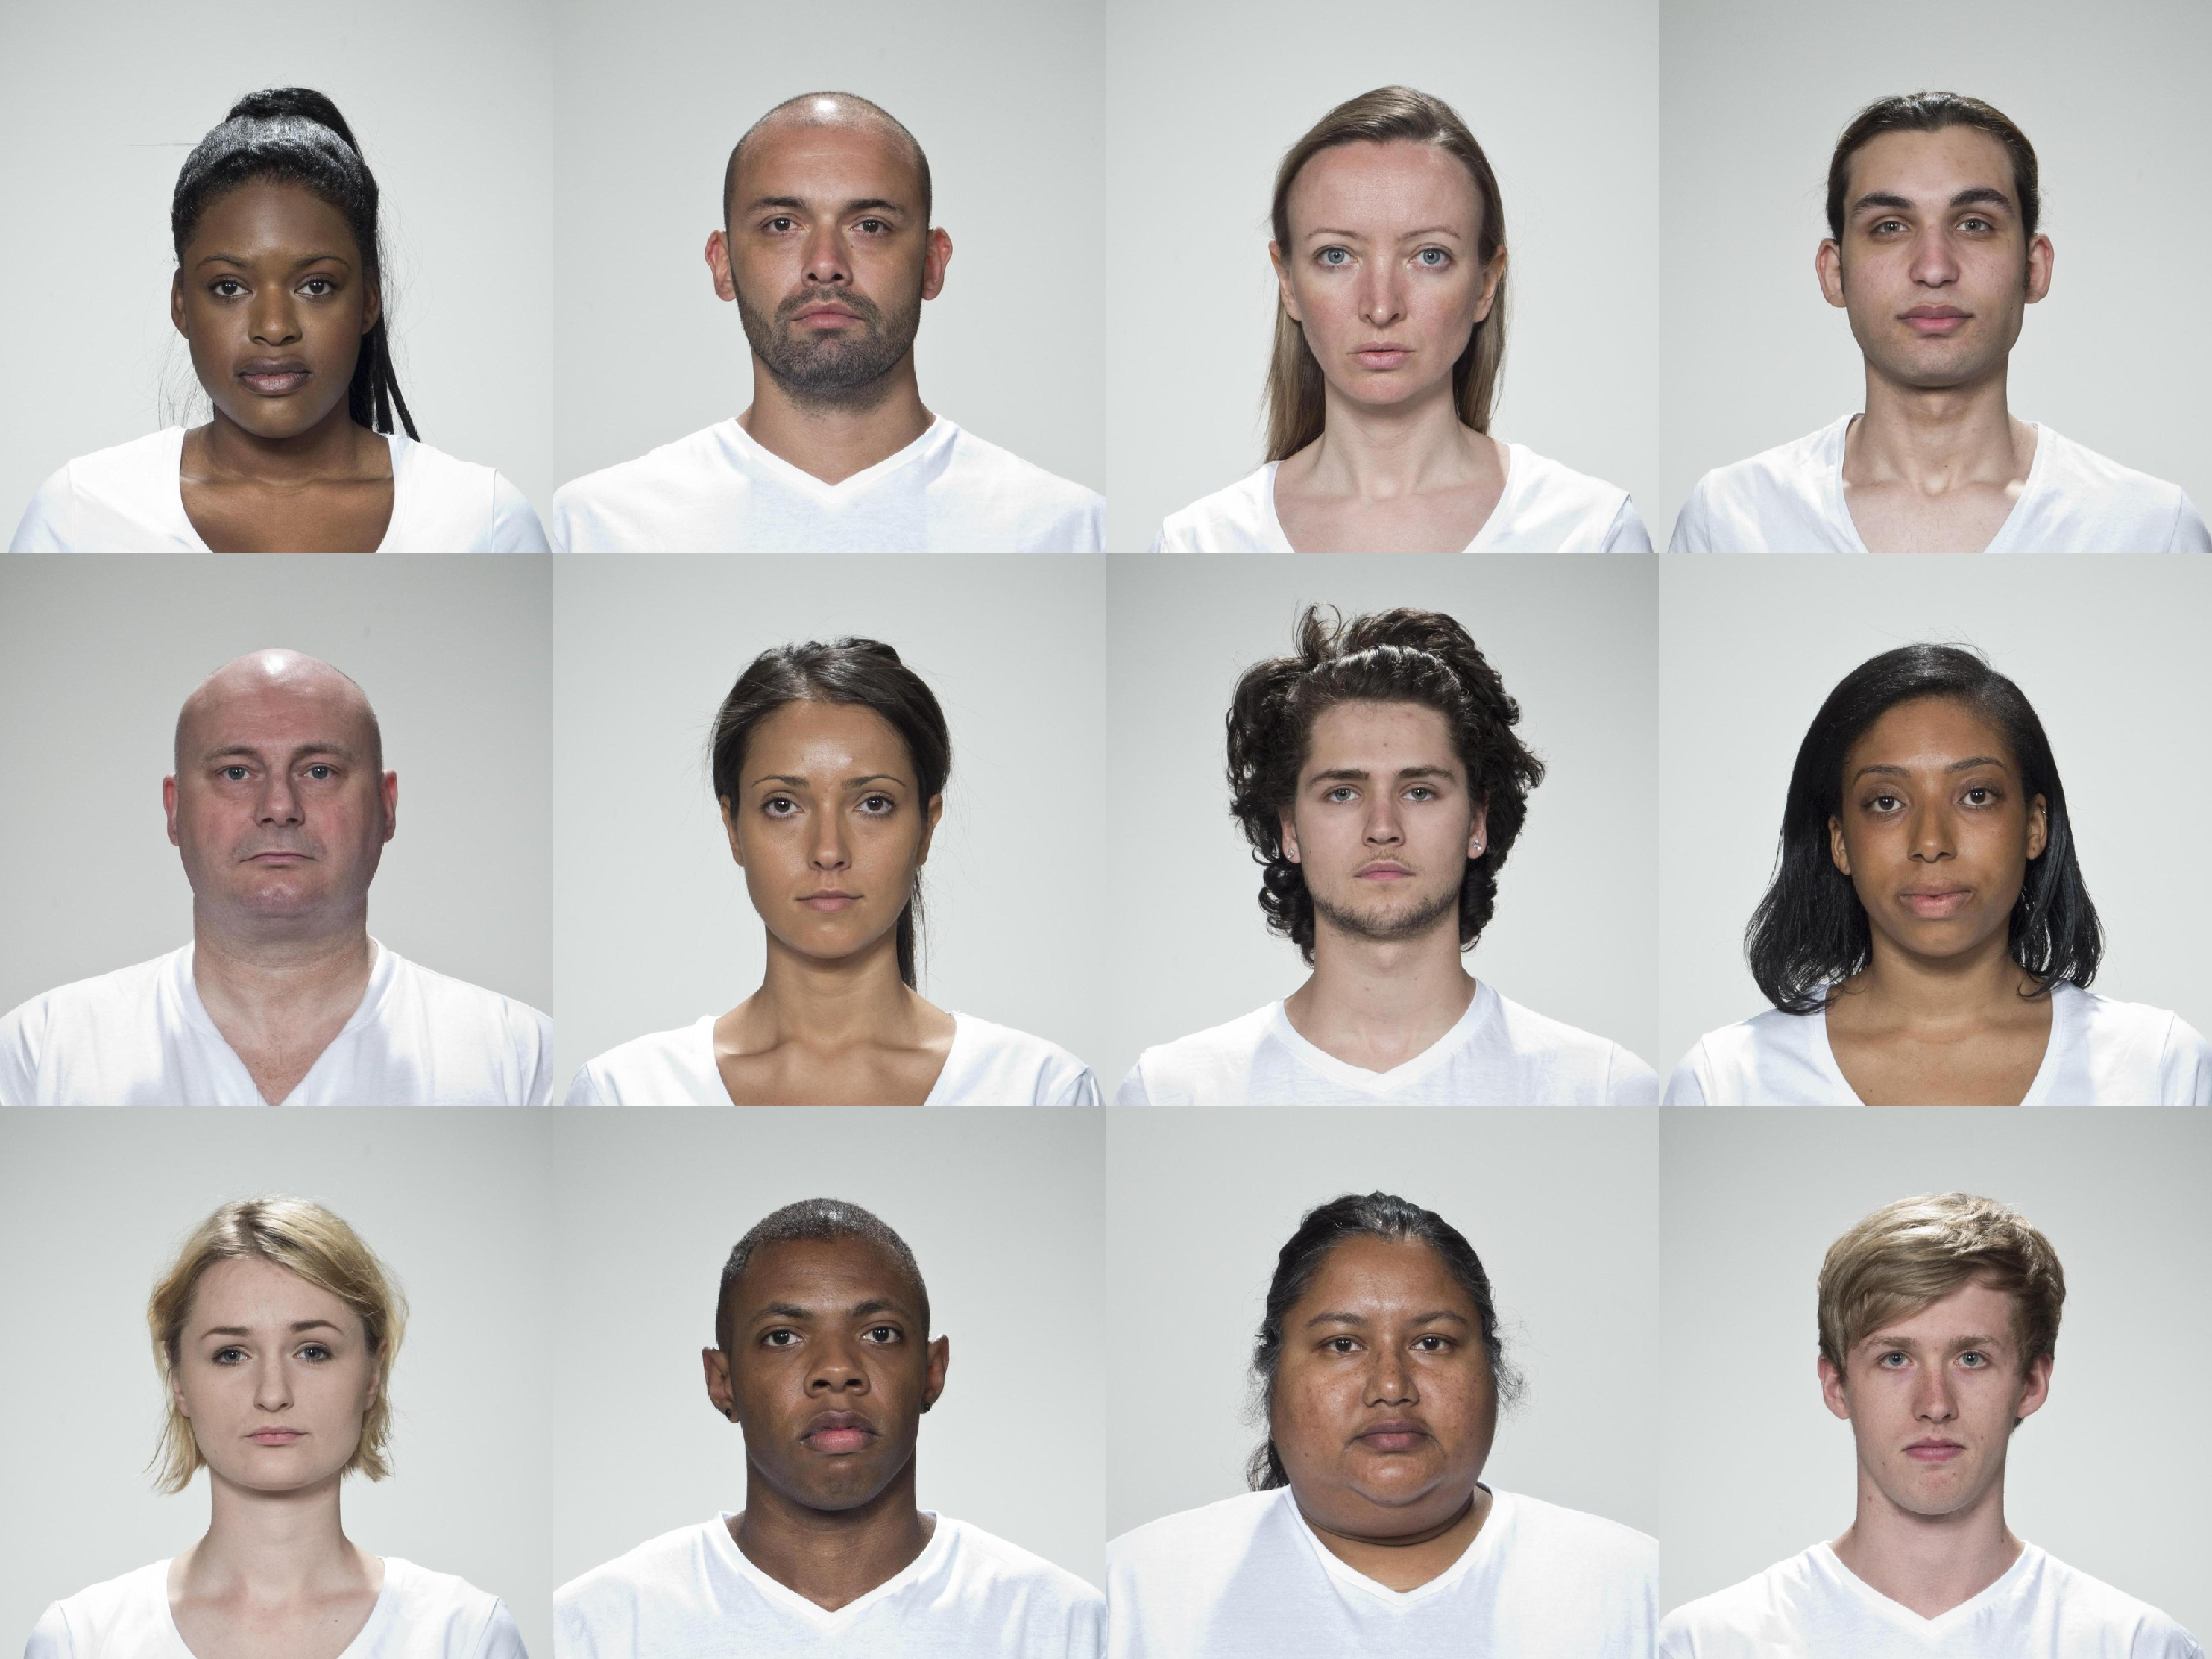
\includegraphics[width=\textwidth]{images/mos_train_set.pdf}\\
        \textbf{(a)} MOS train set % chktex 10
    \end{minipage}
    \hfill
    \begin{minipage}[t]{0.19\textwidth}
        \centering
        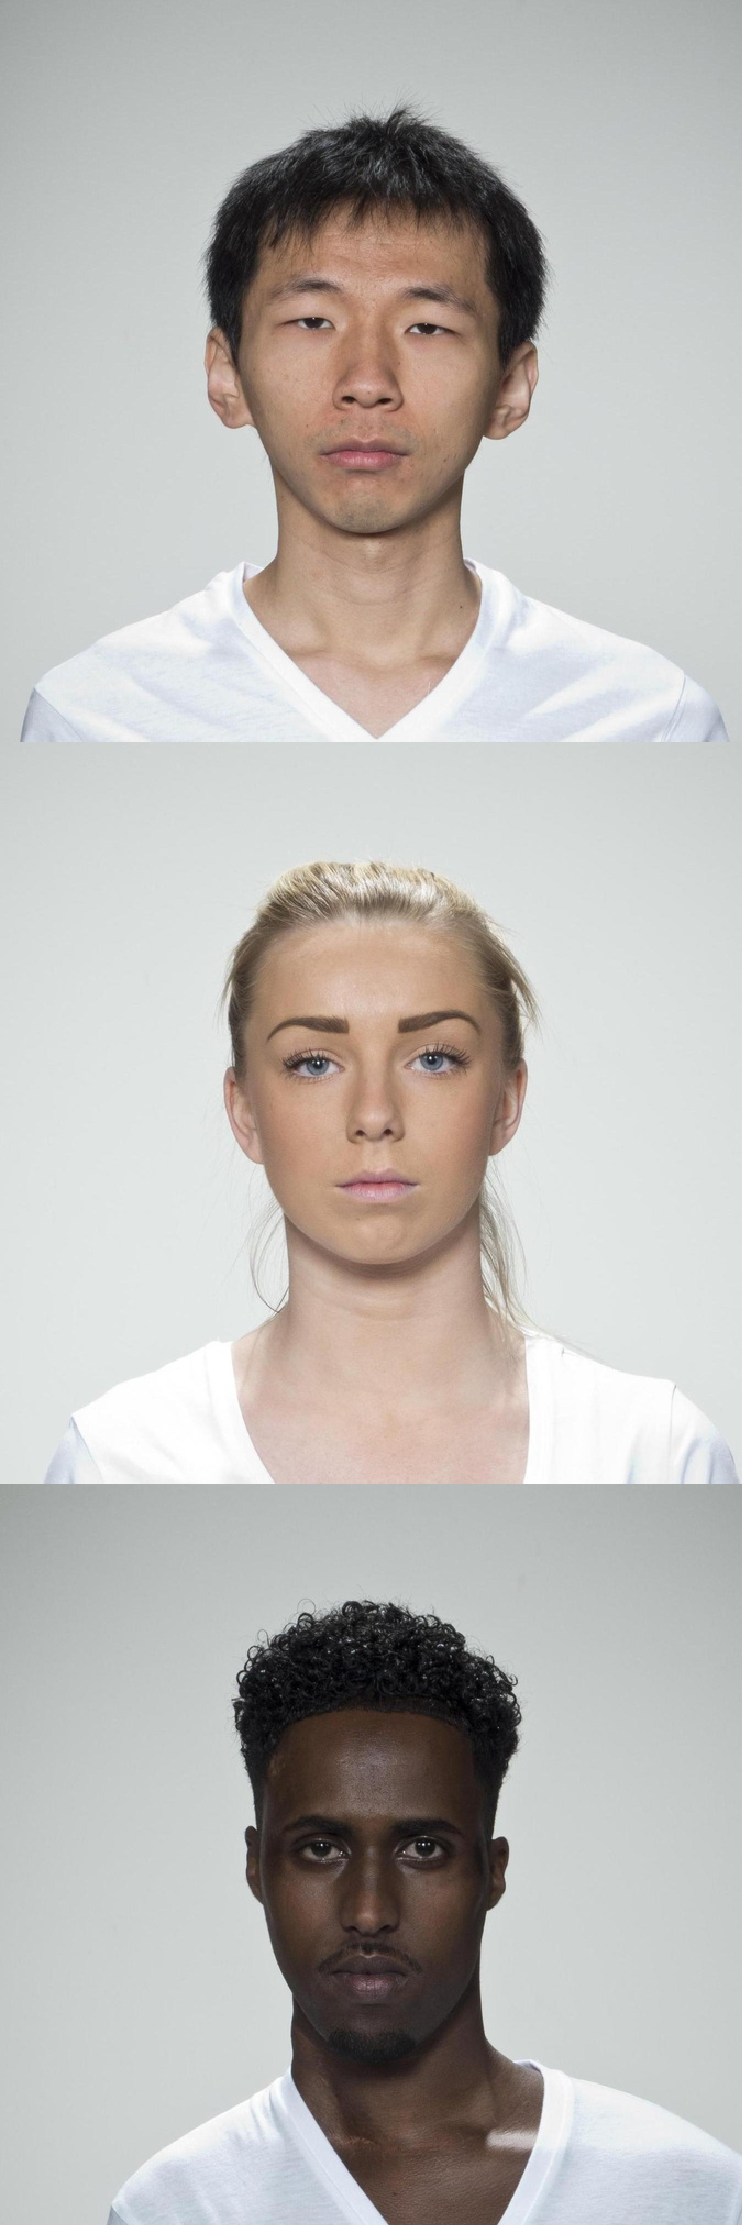
\includegraphics[width=\textwidth]{images/mos_test_set.pdf}\\
        \textbf{(b)} MOS test set % chktex 10
    \end{minipage}
    \caption{Reference images from the MOS set, comprising the selected subjects from the FRLL dataset.}\label{fig:mos_set}
\end{figure}

The printer-proof steganography methods used were based on Generative Adversarial Networks (GANs)~\cite{gans2018} to encode and decode information, illustrated in Fig.~\ref{fig:steganography}. We can obtain various results depending on the method used:

\begin{itemize}
    \item StegaStamp~\cite{stegastamp2020}: claims to be the first steganography model capable of decoding data from printed images. The authors show robust results in decoding data under physical transmission by adding printer noise in the training process.
    \item Code\,Face~\cite{codeface2021}: encoder and decoder networks are trained using end-to-end GANs. It introduces a new security system for encoding and decoding facial images that are printed in common IDs and MRTDs.
    \item RiemStega~\cite{cruz2025riemstega}: proposes a new loss function that extends the loss function based on the $L_2$ distance between images to the Riemannian manifold of symmetric and positive definite matrices.
    \item StampOne~\cite{stampone2024}: focuses on high-level robust steganography, such as~\cite{codeface2021, stegastamp2020}, it balances between high-quality encoded images and decoding accuracy. It mitigates distortion-related issues like JPEG compression, camera sensors and printer's Gaussian noise by incorporating gradient transform and wavelet transform to normalize and balance frequencies of the inputs. 
\end{itemize}

\begin{figure}[ht]
    \centering
    \begin{minipage}[t]{0.2\textwidth}
        \centering
        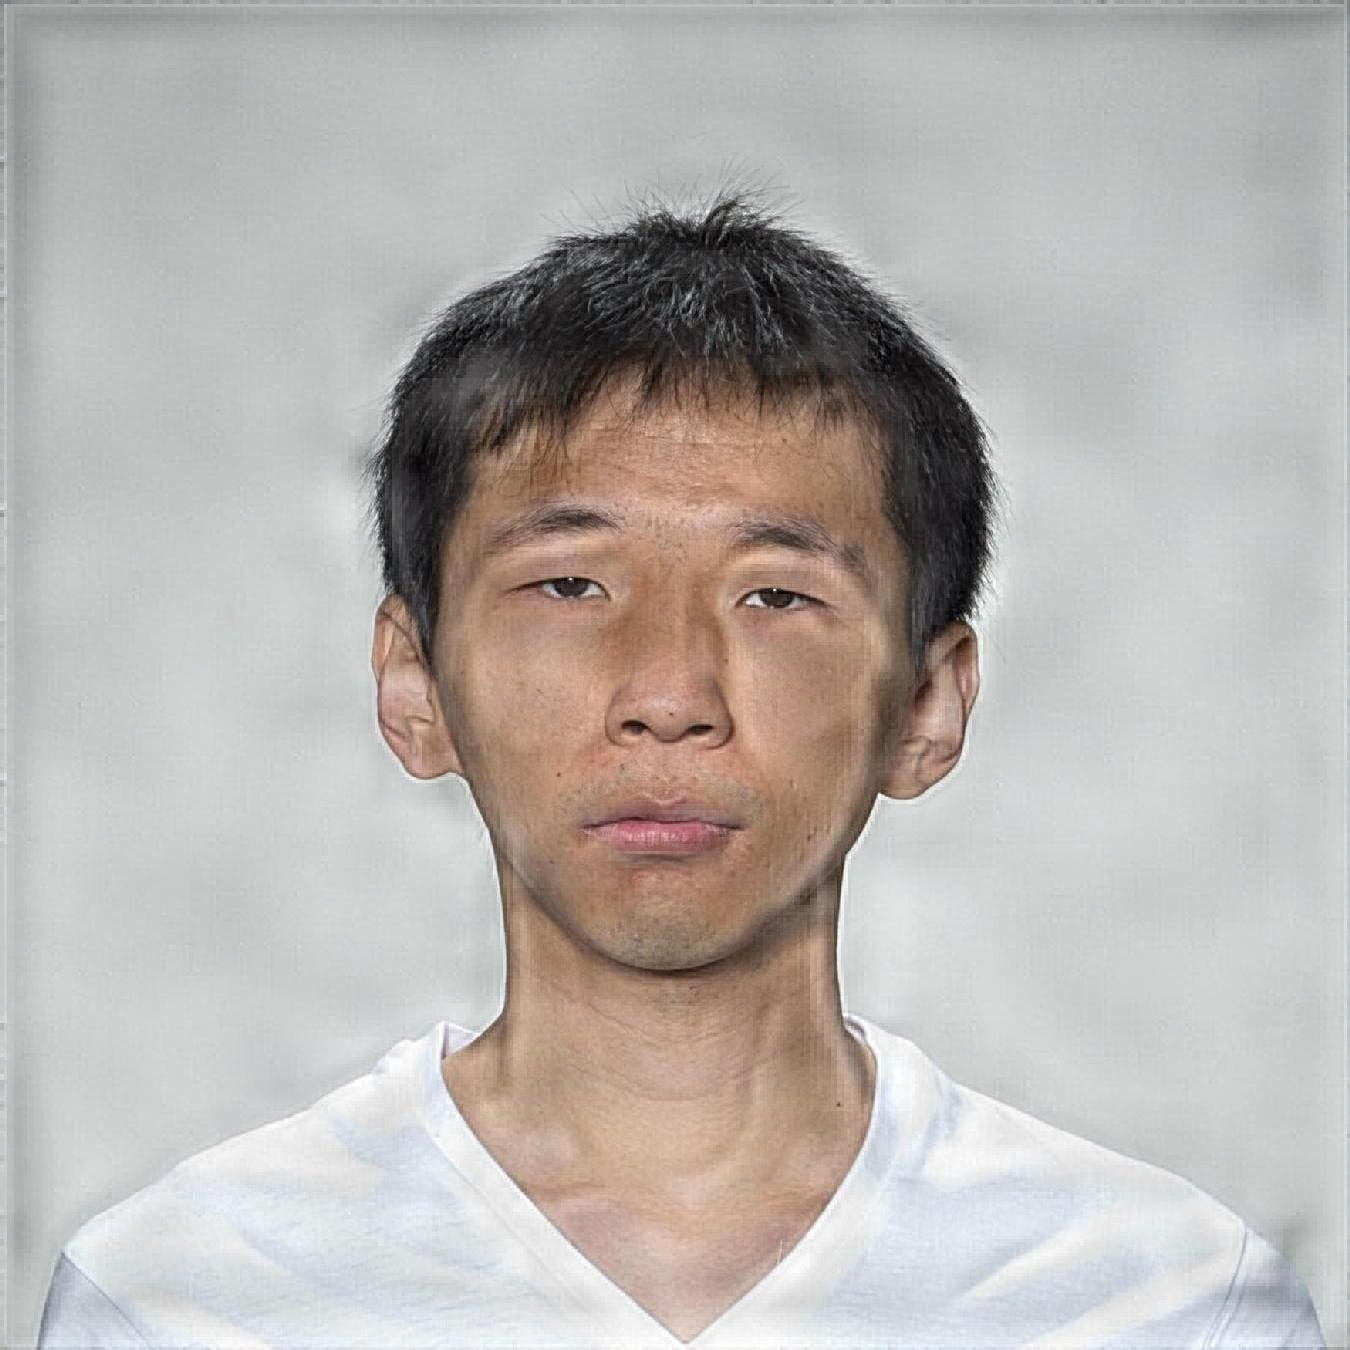
\includegraphics[width=\textwidth]{images/005_StegaStamp_1.4.jpg}\\
        \textbf{(a)} StegaStamp
    \end{minipage}
    \hfill
    \begin{minipage}[t]{0.2\textwidth}
        \centering
        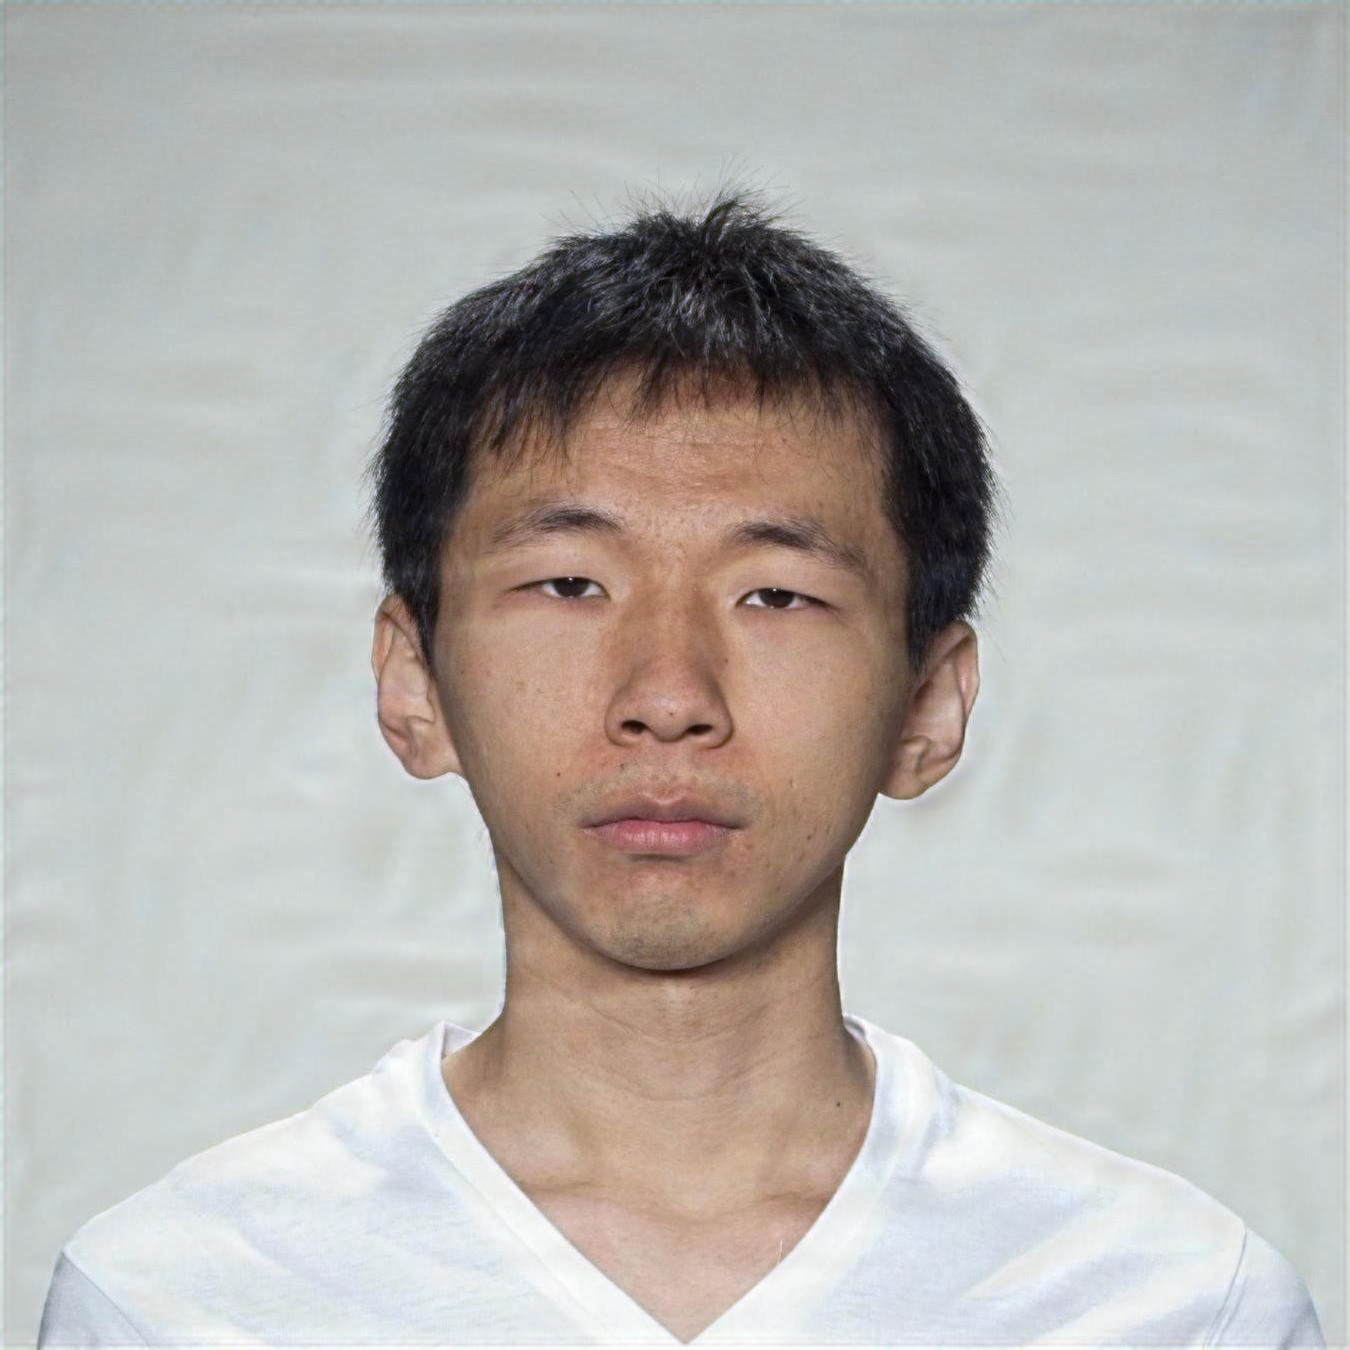
\includegraphics[width=\textwidth]{images/005_CodeFace_1.4.jpg}\\
        \textbf{(b)} Code\,Face
    \end{minipage}
    \hfill
    \begin{minipage}[t]{0.2\textwidth}
        \centering
        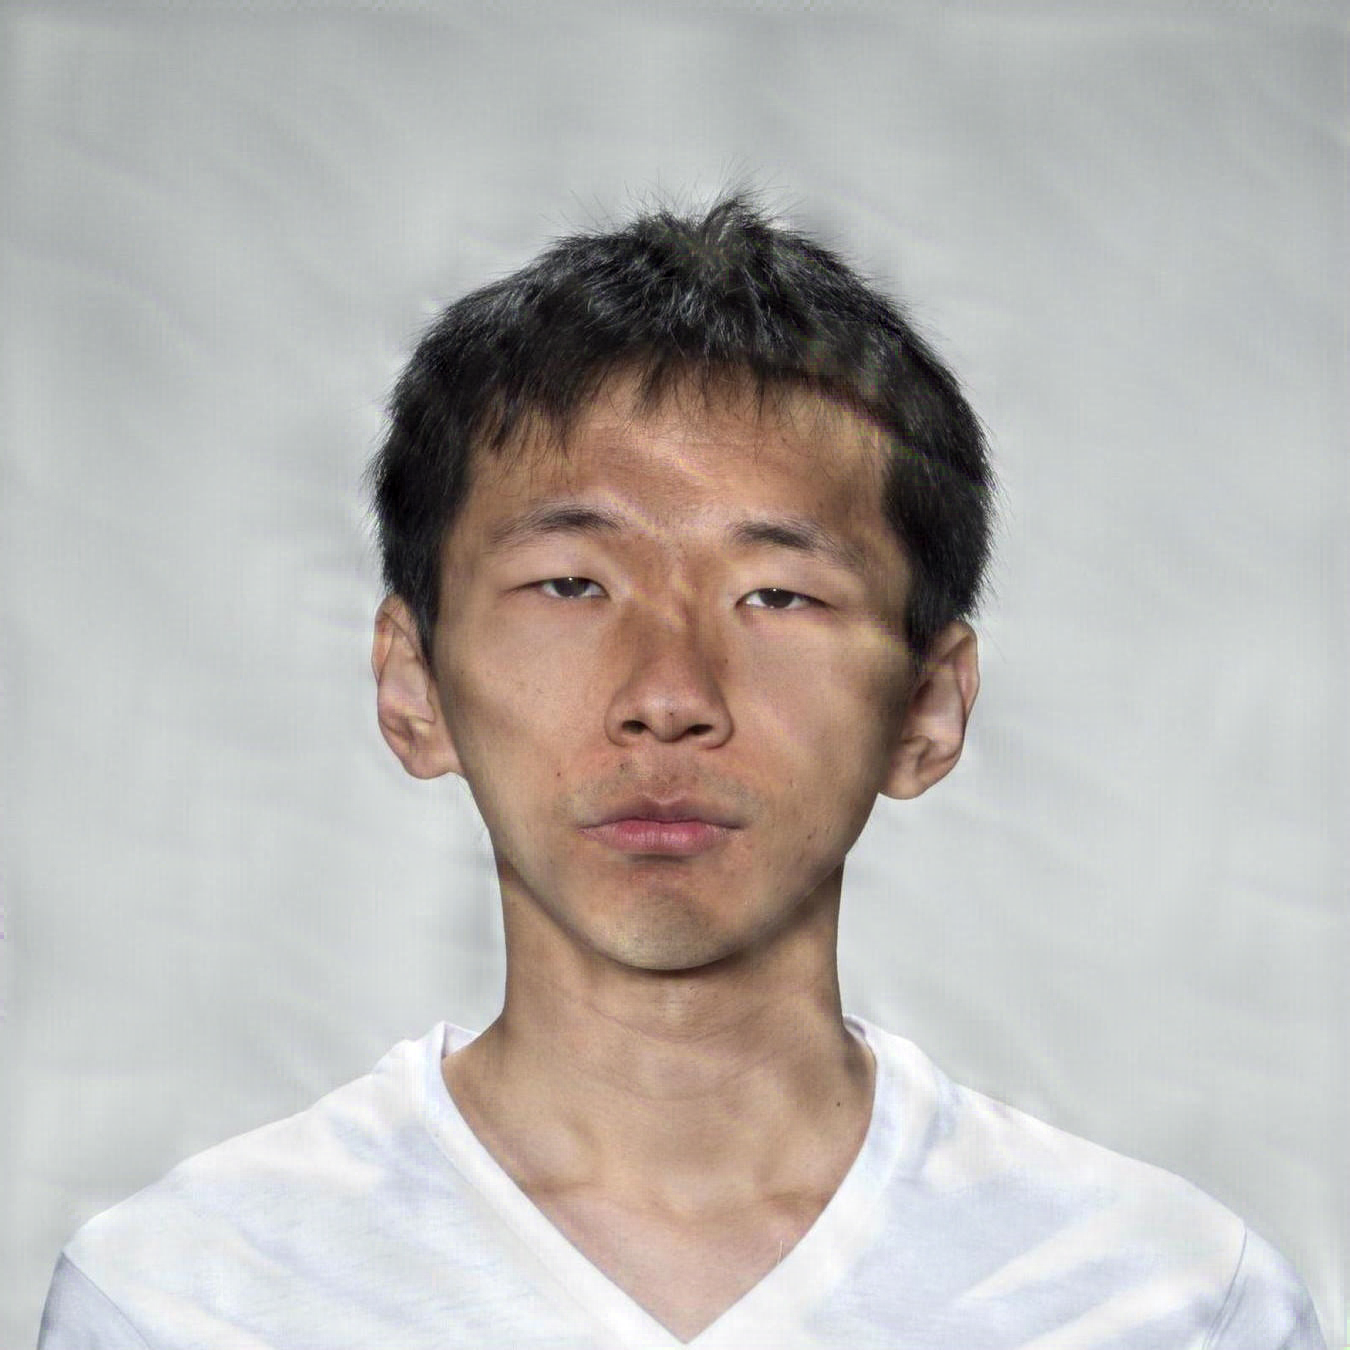
\includegraphics[width=\textwidth]{images/005_RiemStega_1.4.jpg}\\
        \textbf{(c)} RiemStega
    \end{minipage}
    \hfill
    \begin{minipage}[t]{0.2\textwidth}
        \centering
        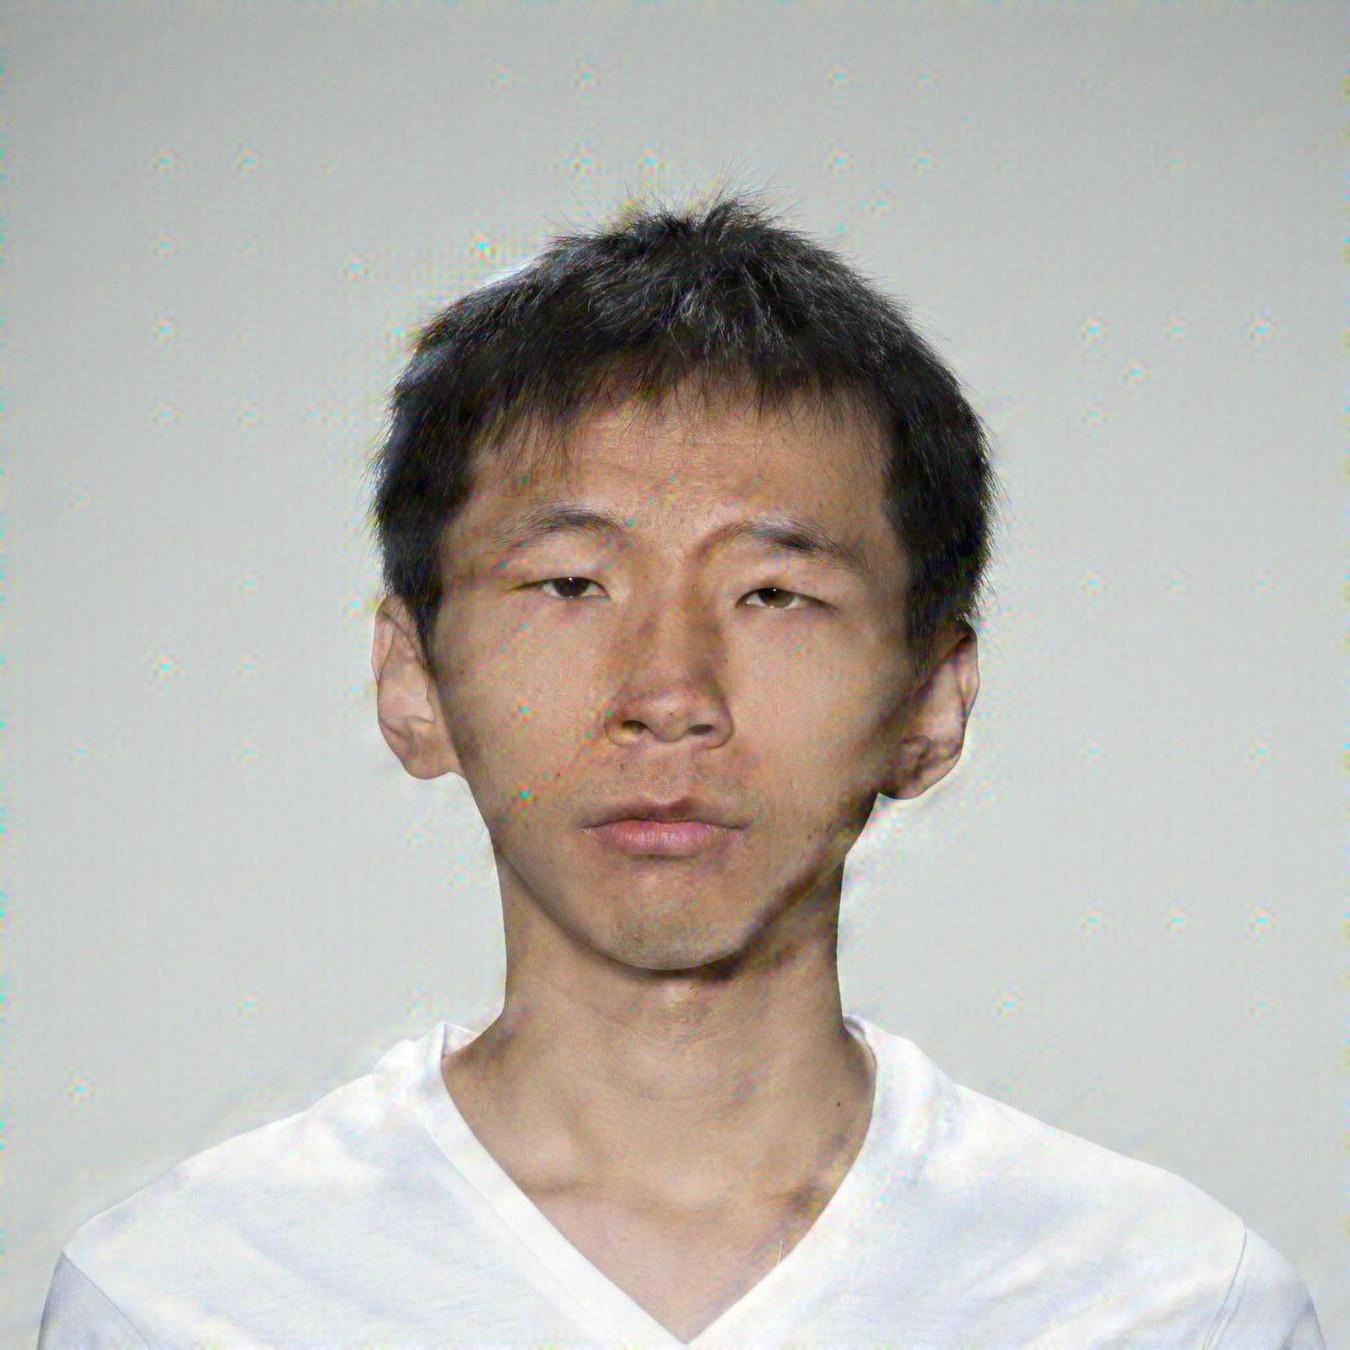
\includegraphics[width=\textwidth]{images/005_StampOne_1.4.jpg}\\
        \textbf{(d)} StampOne
    \end{minipage}
    \caption{Steganographically distorted facial images from each method.}\label{fig:steganography}
\end{figure}


We followed the ITU-R BT.500--15~\cite{ITU-R-BT500} recommendation and adopted the Single Stimulus (SS) method. The test was implemented using a custom Django web application seen in Fig.~\ref{fig:webapp}. Prior to the test session, participants signed an informed consent form and filled out a registration form providing demographic and environmental information such as age, gender, education, country of origin and ethnicity, and others. Each image was shown individually, with no time limit. Ratings were submitted using a labeled slider, and automatic saving ensured session robustness.

Each image in the MOS set was evaluated approximately 30 times by human observers, resulting in over 14,000 ratings. We had around 200 participants, each session lasted about 22 minutes and included roughly 70 evaluations. Following the session, outlier observers were identified and removed using both Kurtosis-based and correlation-based post-screening methods described in ITU-R BT.500--15~\cite{ITU-R-BT500}, resulting in the exclusion of four participants.

\begin{figure}
    \centering
    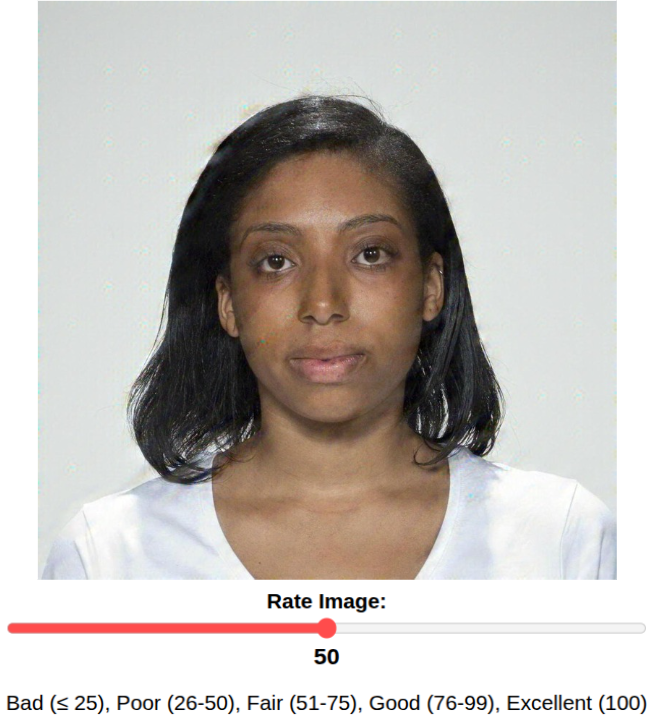
\includegraphics[width=0.32\textwidth]{images/webapp_test.png}
    \caption{Django-based webapp created for the Single Stimulus test.}\label{fig:webapp}
\end{figure}

\subsection{Debiasing of Subjective Scores}

To correct for demographic bias in the subjective scores, we followed a procedure inspired by prior work on bias correction in perceptual tasks~\cite{clapes2018apparent}, where we applied a residualization method based on linear modeling. An ordinary least squares (OLS) regression was fit to the MOS values, using observer and image attributes, and their pairwise interactions as categorical predictors. The fitted bias components were subtracted from the original scores, and the residuals were mean-centered to preserve the global score distribution. As shown in Table~\ref{tab:anova}, several factors exhibit statistically significant effects on the MOS prior to residualization, notably observer and subject ethnicity. After applying the residualization procedure, these effects disappear, as confirmed by an ANOVA test showing no significant impact from any individual factor. The corrected MOS labels are then used as ground truth in all supervised stages of the pipeline to ensure fairness and reduce the influence of socially conditioned priors.

\begin{table}
    \centering
    \caption{ANOVA~\cite{ross2017one} results for observer and image attributes. Before debiasing, several factors show statistically significant effects on MOS, p-value $< 0.05$.\@ After residualization, all main effects show no significant impact, confirming the effectiveness of the debiasing procedure.}\label{tab:anova}
    \begin{tabular}{lcc}
        \toprule
        Factor & p-value & p-value (residualized) \\
        \midrule
        Observer gender                             & 0.022                 & 0.9930 \\
        Observer ethnicity                          & $8.44 \times 10^{-4}$ & 1 \\
        Subject gender                              & $1.60 \times 10^{-3}$ & 0.9722 \\
        Subject ethnicity                           & $7.36 \times 10^{-3}$ & 1 \\
        Observer gender $\times$ Subject gender     & 0.6417              & 0.6417 \\
        Observer ethnicity $\times$ Subject ethnicity & 0.0582              & 0.0582 \\
        \bottomrule
    \end{tabular}
\end{table}

\subsection{Correlation of FR-IQA Metrics with Human Perception}

We compute 40 FR-IQA scores for each distorted image in the dataset and compare them against the corresponding MOS, as seen in Fig.~\ref{fig:mos_vs_iqa}. Several metrics exhibit strong linear trends with MOS, while others are poorly aligned or even negatively correlated. For a detailed description of these metrics, we refer the reader to~\cite{shahrukh2019survey}.



\begin{figure}
    \centering
    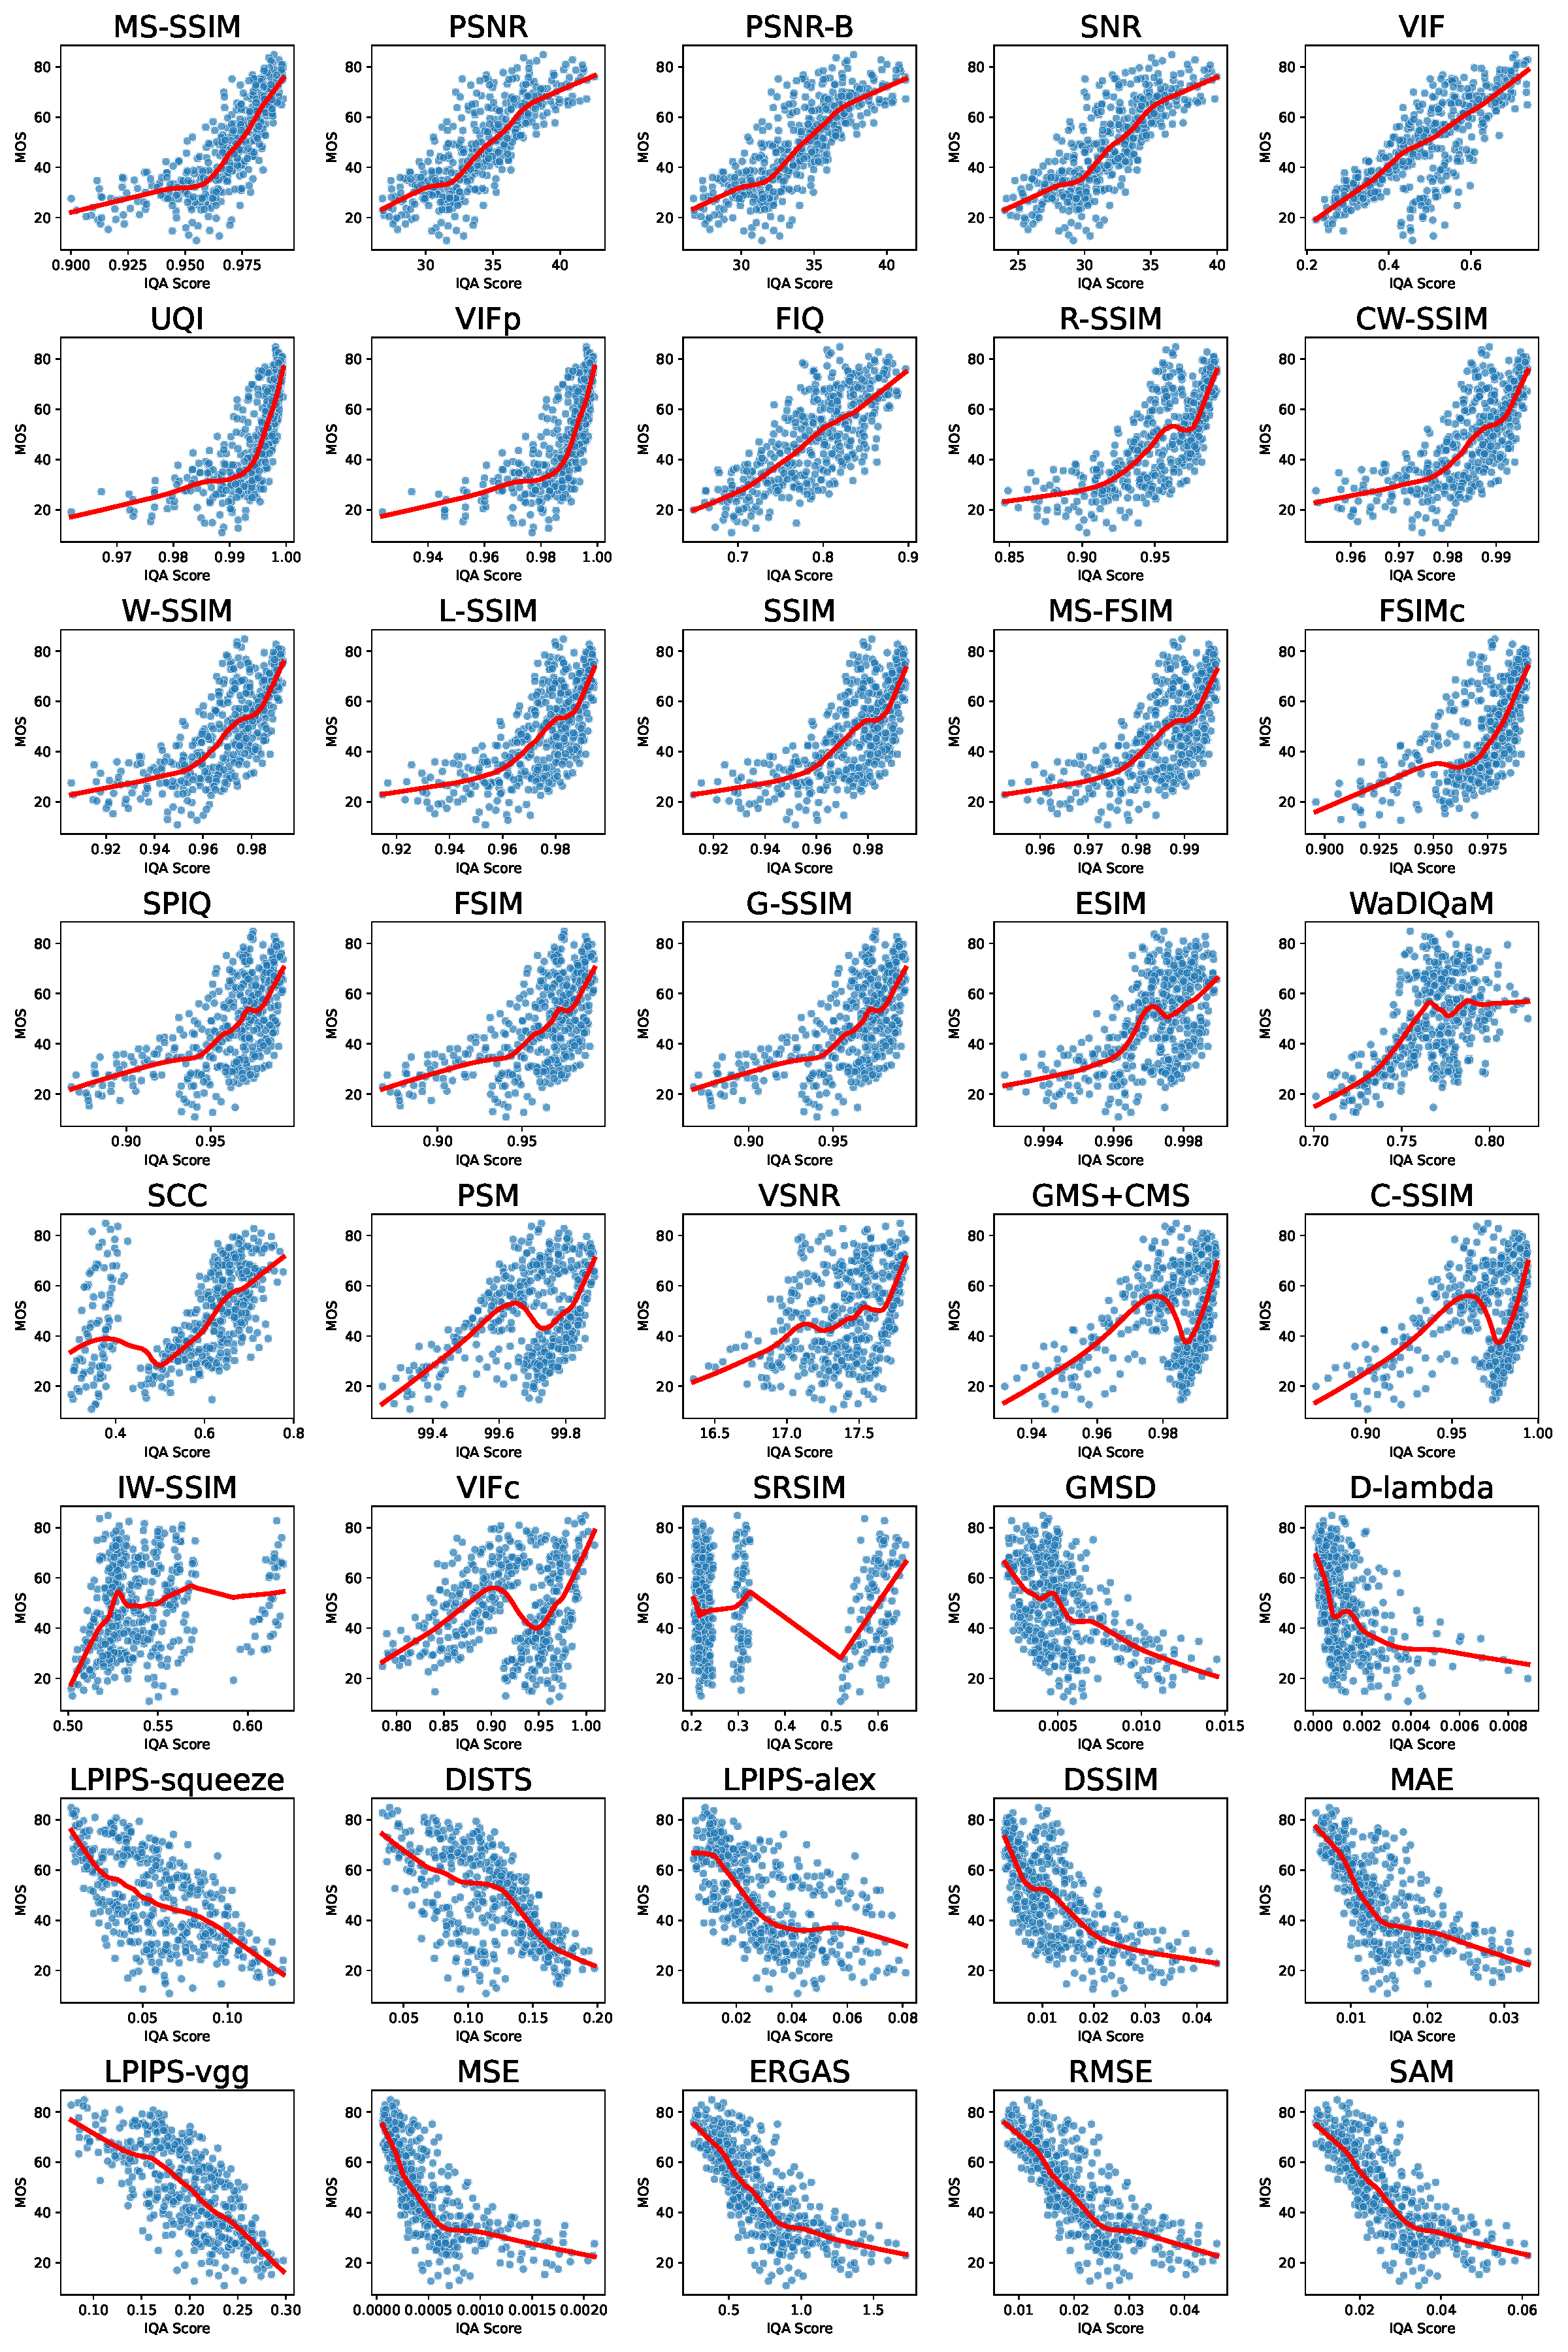
\includegraphics[width=0.98\linewidth]{images/mos_vs_iqa_grid.pdf}
    \caption{Scatter plots illustrating the relationship between MOS and 40 individual full-reference IQA metrics. The red line represents a smoothed local trend curve.}\label{fig:mos_vs_iqa}
\end{figure}

\subsection{Fusion of FR-IQA Metrics for Pseudo-MOS Estimation}

To identify which metrics align best with human perception, we compute both the Pearson Linear Correlation Coefficient (PLCC) and the Spearman Rank-Order Correlation Coefficient (SRCC)~\cite{plcc-srcc} which respectively quantify the linearity and monotonicity of the relationship between metric scores and MOS.\@ To determine the appropriate number of metrics to retain for fusion, we applied Singular Value Decomposition (SVD) and the Picard criterion~\cite{hansen1998picard}. Metrics are first ranked by the average of their PLCC and SRCC with MOS.\@ After normalizing the feature matrix, SVD revealed that six components capture 95\% of the total variance, as shown in Fig.~\ref{fig:svd_analysis}a, indicating an optimal dimensionality of $k=6$.

To validate this truncation point, we examined the Picard plot in Fig.~\ref{fig:svd_analysis}b, which compares singular values with the target projections. The stable ratio in the tail confirms that six components provide a good balance between expressiveness and stability. This supports a compact, informative subset of FR-IQA metrics.

\begin{figure}[ht]
    \centering
    \begin{minipage}[t]{0.48\textwidth}
        \centering
        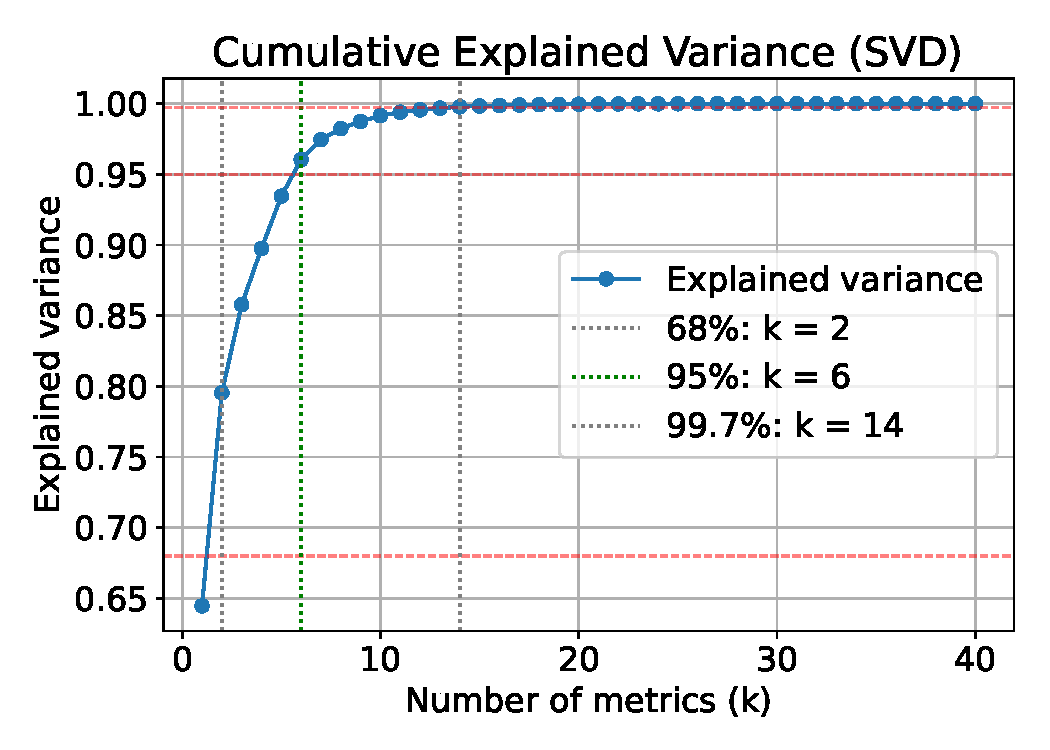
\includegraphics[width=\linewidth]{images/variance.pdf}
        \textbf{(a)} Cumulative variance explained by SVD components.
    \end{minipage}
    \hfill
    \begin{minipage}[t]{0.48\textwidth}
        \centering
        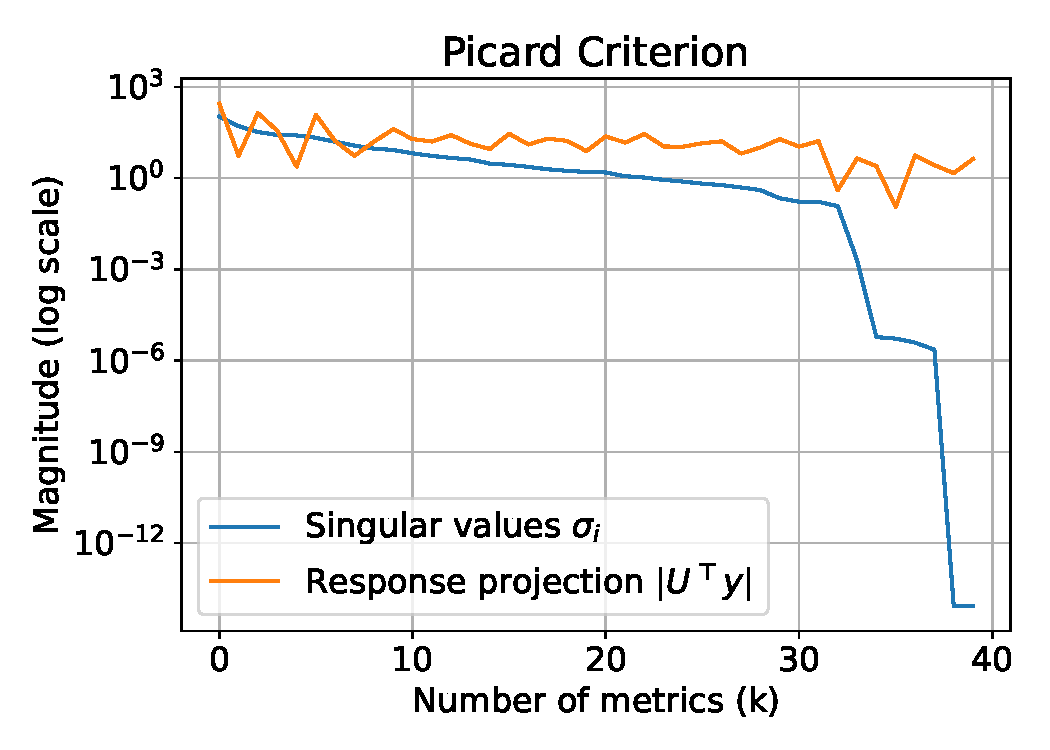
\includegraphics[width=\linewidth]{images/picard.pdf}
        \textbf{(b)} Magnitude of singular values and projected response.
    \end{minipage}
    \caption{SVD-based analysis of the FR metric space. The cumulative explained variance (a) guides the choice of dimensionality, while the Picard criterion (b) illustrates stability near $k=6$.}\label{fig:svd_analysis}
\end{figure}

After selecting the top $k = 6$ FR-IQA metrics, we trained a diverse set of supervised regressors to map these features to subjective MOS scores. The models included both linear and non-linear types:

\begin{itemize}
    \item Linear models: Linear Regression~\cite{linearregression}, Ridge Regression~\cite{ridgeregression}, Bayesian Ridge~\cite{bayesianridge}, ElasticNet~\cite{elasticnet}.
    \item Kernel-based: Support Vector Regression~\cite{svr} (SVR).
    \item Ensembles: Random Forest~\cite{randomforest}, Extra Trees~\cite{ensembles}, Gradient Boosting~\cite{gradboosting}, HistGradientBoosting~\cite{histboost}.
    \item Boosted Trees: XGBoost\cite{xgboost}, LightGBM~\cite{lightgbm}, CatBoost~\cite{catboost}.
\end{itemize}

Each regressor was trained using five-fold cross-validation with an exhaustive grid search over predefined hyperparameter spaces. The best model, CatBoost, optimal configuration was: depth = 8, iterations = 500, learning rate = 0.05, and $L_2$ regularization = 1. This trained regressor is then applied to the unlabeled portion of the dataset (3,132 distorted images), generating pseudo-MOS.\@

\subsection{Training a No-Reference IQA Model from Pseudo-MOS}

To enable NR quality prediction, we train a deep regression model end-to-end using pseudo-MOS scores as targets. The architecture is based on a ResNet-18 backbone~\cite{resnet} pretrained on ImageNet~\cite{imagenet}, with its final classification layer replaced by a lightweight multi-layer perceptron (MLP) regressor~\cite{bayesianridge}. All layers are fine-tuned during training to learn perceptual quality representations specific to our task. The training set consists of distorted facial images paired with either pseudo-MOS, from the FR fusion, or real MOS labels, when available. The model is optimized using MSE and evaluated on the disjoint MOS test set of labeled images. Once trained, the model infers image quality solely from the distorted input, enabling NR assessment aligned with human perception.


\section{Results}

\subsection{Correlation of Individual IQA Metrics with Human Perception}

The correlation analysis between individual FR-IQA metrics and human-rated MOS revealed substantial variability in performance. As shown in Fig.~\ref{fig:mos_vs_iqa}, several metrics exhibit strong linear trends with MOS, while others are poorly aligned or even negatively correlated. To quantify this, we ranked all 41 metrics based on the average of their PLCC and SRCC.\@

Fig.~\ref{fig:ranking} presents this ranking, highlighting that metrics such as PSNR, PSNR-B~\cite{ma2011psnr}, and MS-SSIM~\cite{wang2003multiscale} show the highest alignment with subjective opinion, while others, such as SRSIM~\cite{wang2004image}, diverge significantly.


\begin{figure}
    \centering
    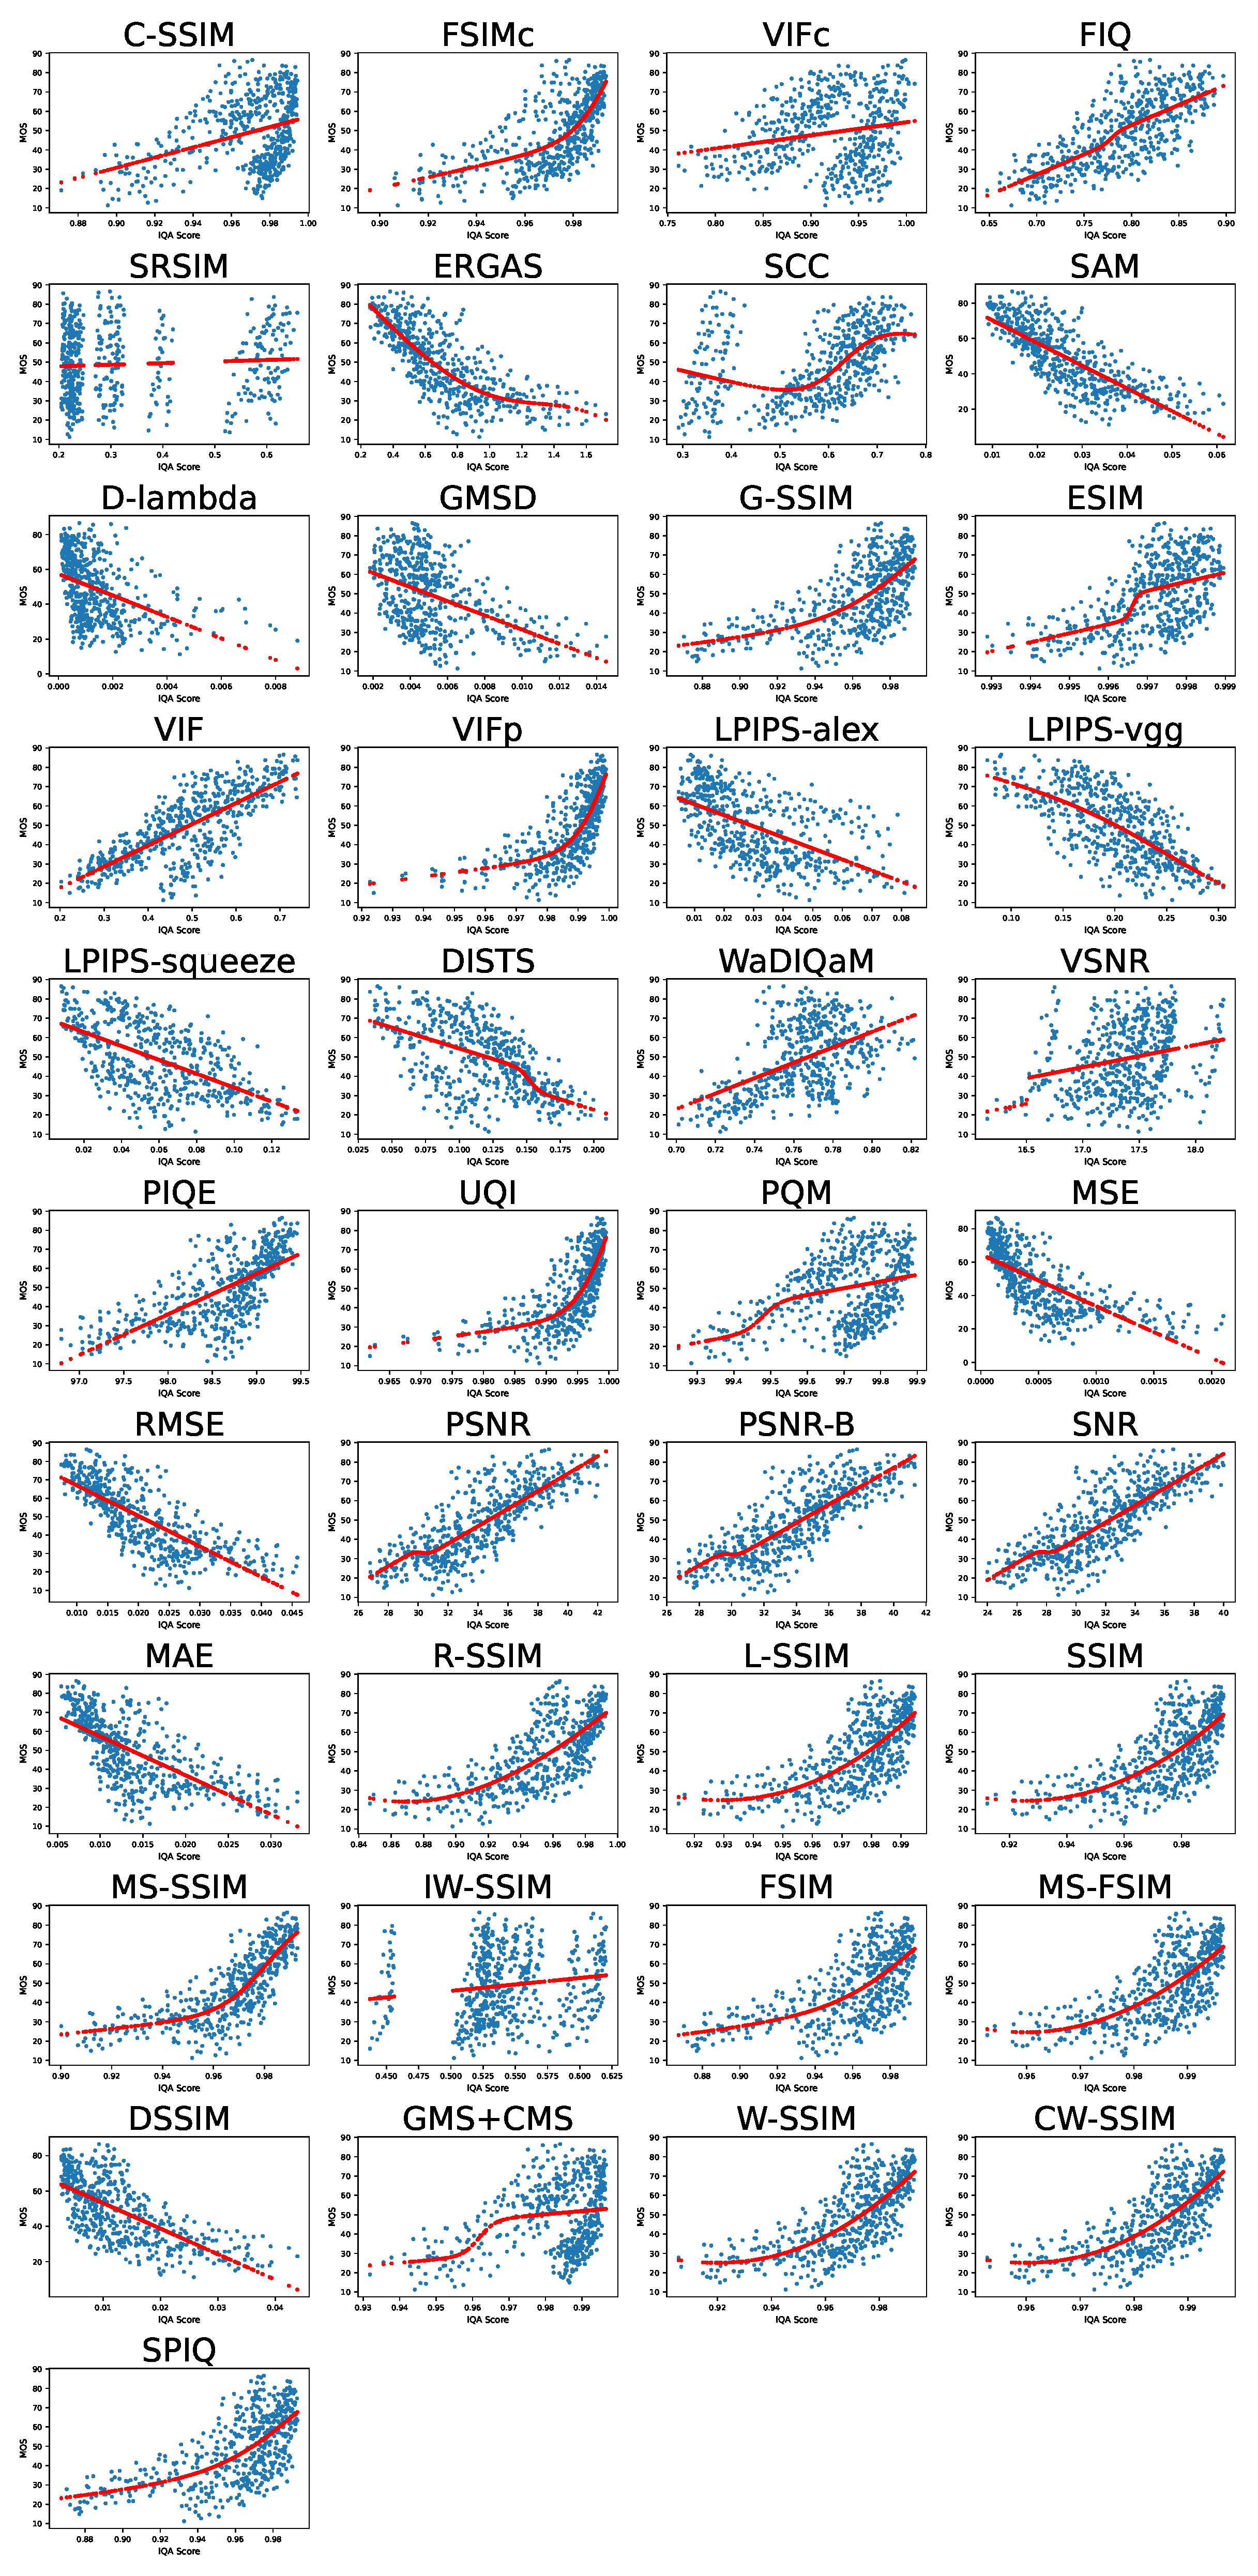
\includegraphics[width=0.7\linewidth]{images/mos_vs_iqa_grid.eps}
    \caption{Scatter plots illustrating the relationship between Mean Opinion Scores (MOS) and individual Full-Reference IQA metrics.}\label{fig:mos_vs_iqa}
\end{figure}

\begin{figure}
    \centering
    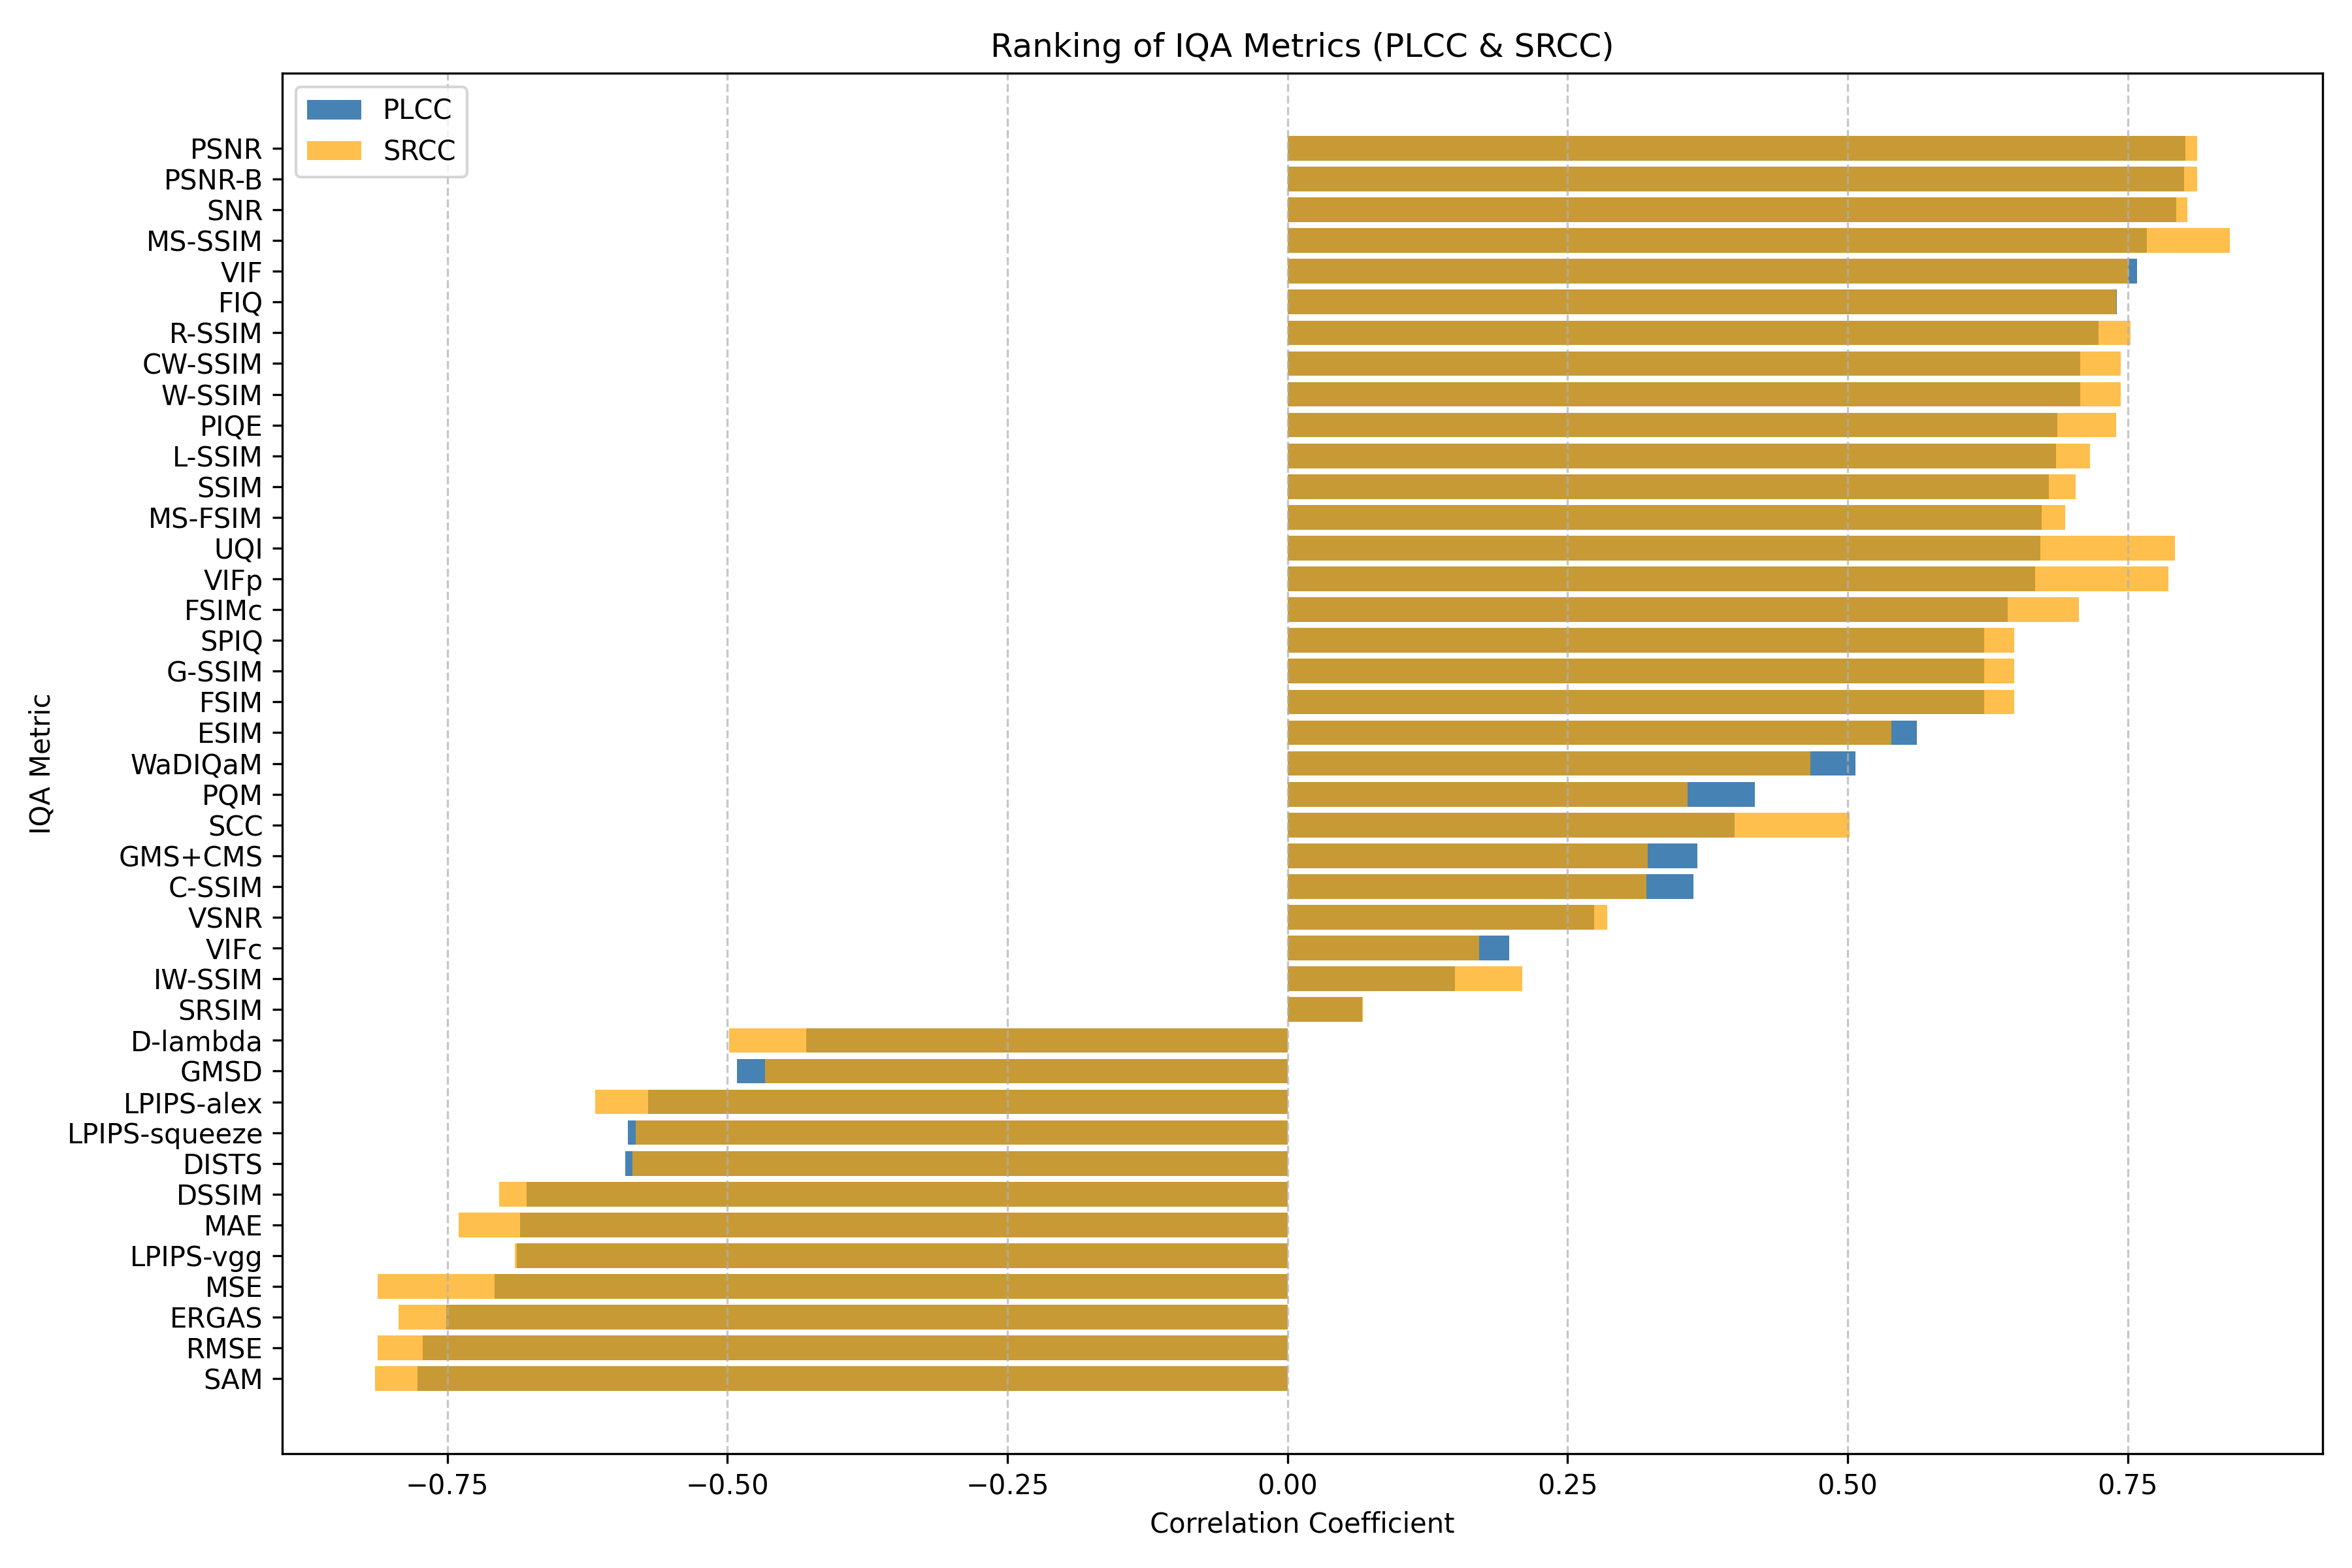
\includegraphics[width=0.9\linewidth]{images/metrics_bar.png}
    \caption{Ranking of FR-IQA metrics by correlation with MOS (PLCC and SRCC).}\label{fig:ranking}
\end{figure}

\subsection{Full-Reference Fusion Performance}

Using the 432 MOS-labeled images and $k = 5$ best metrics, we evaluated six fusion models.

As summarized in Table~\ref{tab:fusion_scores}, the Random Forest regressor achieved the best overall performance across all four evaluation metrics, as seen in Fig.~\ref{fig:randomforest}. Notably, it reached a PLCC of 0.8582 and SRCC of 0.8637, outperforming both linear and gradient boosting approaches.

\begin{figure}
    \centering
    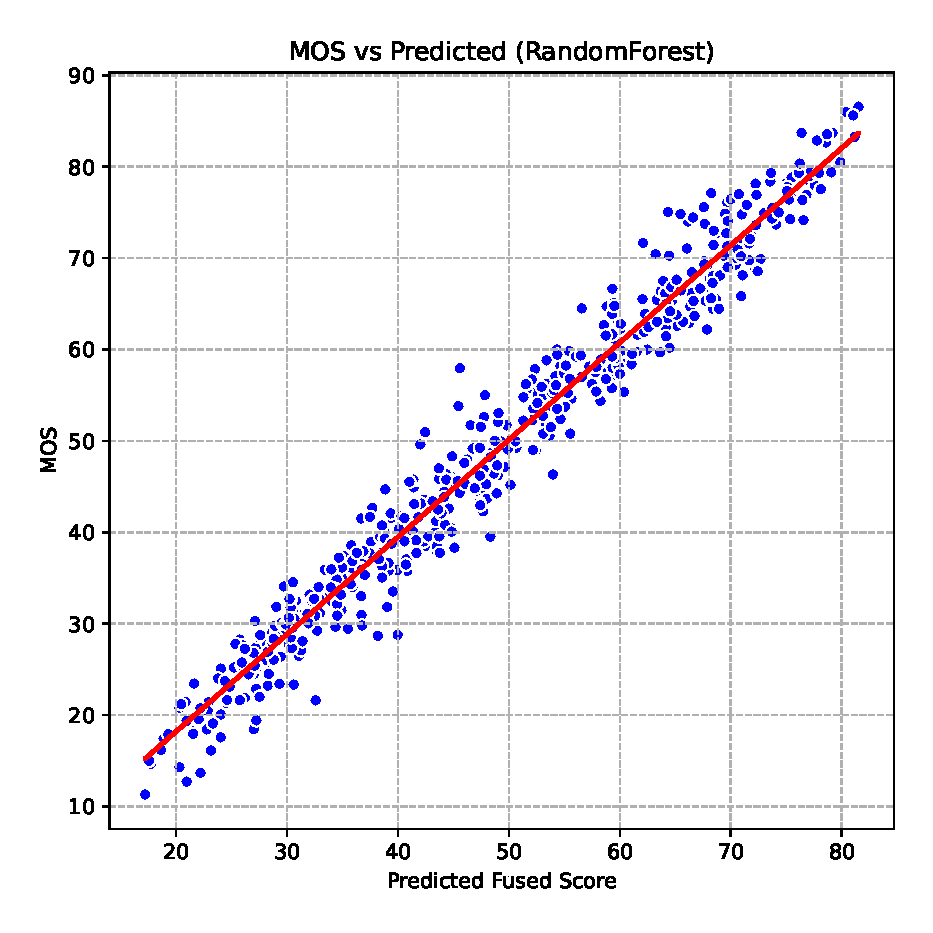
\includegraphics[width=0.6\linewidth]{images/fusion_plot_RandomForest.eps}
    \caption{MOS vs. Predicted fused Random Forest score}\label{fig:randomforest}
\end{figure}

\begin{table}
\caption{Fusion performance on 432 labeled images (MOS ground truth).}
\begin{center}
\begin{tabular}{lcccc}
\toprule
\textbf{Model} & \textbf{PLCC} & \textbf{SRCC} & \textbf{MSE} & \textbf{MAE} \\
\midrule
Linear Regression & 0.8123 & 0.8248 & 108.83 & 7.98 \\
Ridge             & 0.8125 & 0.8246 & 108.76 & 7.96 \\
Random Forest     & \textbf{0.8582} & \textbf{0.8637} & \textbf{84.48}  & \textbf{6.95} \\
SVR               & 0.8207 & 0.8207 & 108.44 & 8.08 \\
XGBoost           & 0.8560 & 0.8596 & 108.44 & 8.08 \\
LightGBM          & 0.8560 & 0.8577 & 85.90  & 7.15 \\
\bottomrule
\end{tabular}\label{tab:fusion_scores}
\end{center}
\end{table}

The trained Random Forest model was then applied to 3,132 unlabeled images, generating pseudo-MOS scores that serve as soft ground truth for the no-reference model.

\subsection{No-Reference Regression Model}

We trained a NR regressor using features extracted from a ResNet-18 pretrained on ImageNet. These features, paired with the pseudo-MOS scores generated from the fusion model, served as training data for a second Random Forest model.

Fig.~\ref{fig:nr_vs_fusion} shows the resulting alignment between the predicted NR quality scores and the fusion-based pseudo-MOS values. A clear linear trend is observed, with the model capturing both low and high quality regimes effectively.

\begin{figure}
    \centering
    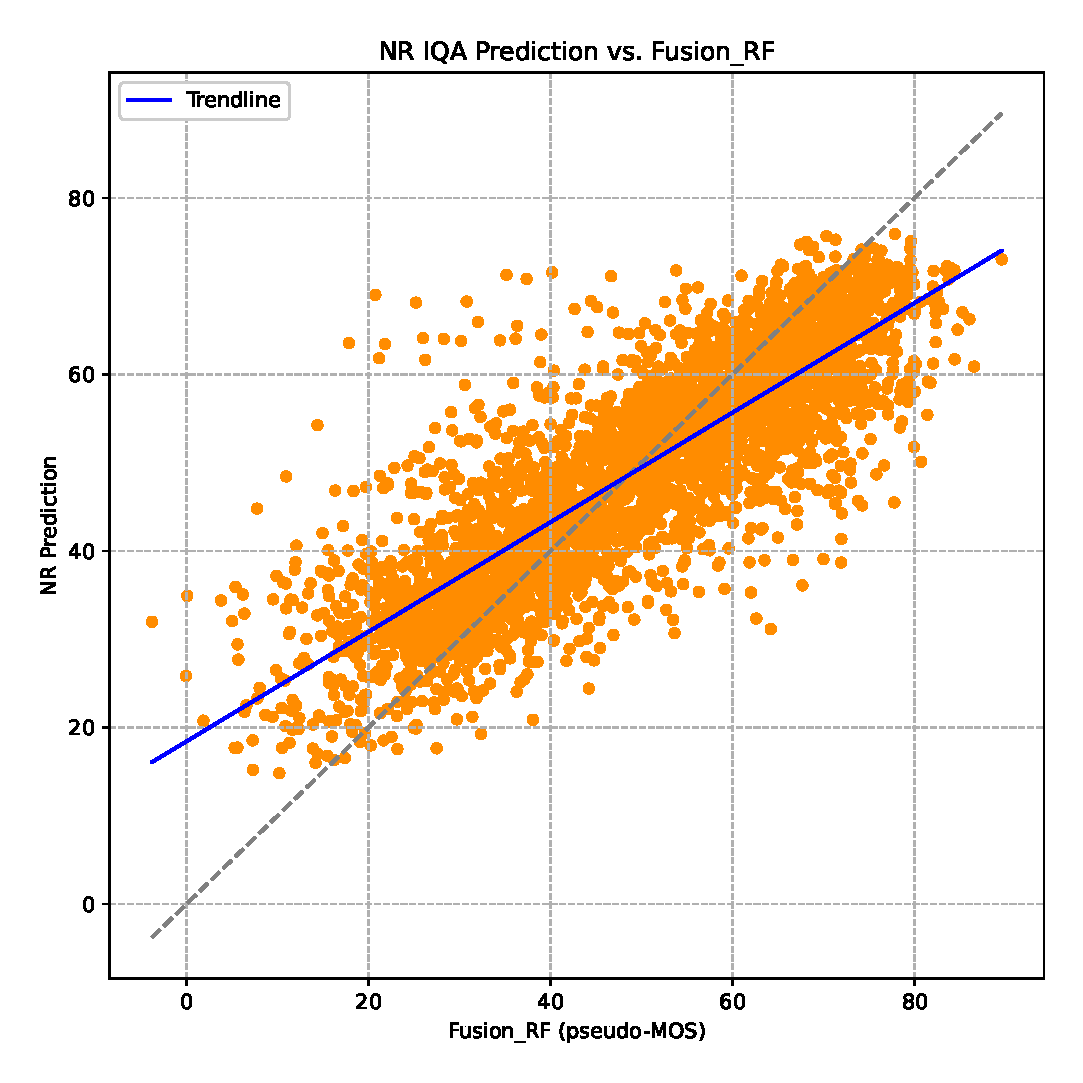
\includegraphics[width=0.6\linewidth]{images/nr_vs_fusion_rf.eps}
    \caption{Scatter plot of NR predictions vs.\ pseudo-MOS scores. The dashed line indicates identity; the blue line is the linear trend.}\label{fig:nr_vs_fusion}
\end{figure}

Quantitative results are reported in Table~\ref{tab:nr_scores}. Our proposed model, trained using deep features and pseudo-MOS supervision, achieves a PLCC of 0.8361 and SRCC of 0.8382, with an MSE of 90.48 and MAE of 7.16. In comparison, classical NR metrics such as NIQE and PIQE demonstrate weaker correlations with perceptual quality and substantially higher error. Even task-specific approaches like SER-FIQ and MagFace underperform, highlighting the robustness of our weakly supervised strategy for NR-IQA on steganographically degraded facial images.

\begin{table}
\caption{Performance of our NR IQA model, ResNet18 + Random Forest (RF), compared to standard NR-IQA baselines, using pseudo-MOS as ground truth.}
\begin{center}
\begin{tabular}{lcccc}
\toprule
\textbf{Method} & \textbf{PLCC} & \textbf{SRCC} & \textbf{MSE} & \textbf{MAE} \\
\midrule
Ours (ResNet18 + RF) & \textbf{0.8361} & \textbf{0.8382} & \textbf{90.48} & \textbf{7.16} \\
NIQE                 & 0.7536          & 0.7431          & 6859.81        & 82.62 \\
PIQE                 & 0.2993          & 0.3114          & 3297.65        & 57.05 \\
SER-FIQ              & -0.1648         & -0.1542         & 123.50         & 9.23 \\
MagFace              & -0.6095         & -0.6362         & 4437.91        & 66.24 \\
\bottomrule
\end{tabular}\label{tab:nr_scores}
\end{center}
\end{table}


\section{Conclusion and Future Work}

Beyond the evaluation of IQA metrics and fusion methods, this study analyzed the extent of observer demographic biases in MOS ratings. The ANOVA results presented in Section~\ref{sec:methodology} indicate that observer characteristics, including gender, ethnicity, and country of origin, significantly influenced MOS.\@ These findings suggest that FIQA methodologies should account for potential biases introduced by subjective assessments from diverse observer groups.

A promising direction for future research is the development of a fully automated, no-reference ICAO-compliant image quality assessment model. Our current approach relies on a fusion of full-reference IQA metrics, which requires access to pristine reference images for quality comparison. However, in real-world applications, such as passport verification and ID issuance, reference images are often unavailable. To address this limitation, we propose training a deep neural network (DNN) on the fusion metric, enabling the transition from a reference-based to a no-reference image quality model.

Developing a deep learning-based, no-reference ICAO-compliant IQA model represents a crucial step toward improving image quality evaluation in biometric and security applications. This approach would ensure robust, unbiased, and practical quality assessments for automated identity verification systems.

\bibliographystyle{splncs04}
\bibliography{references}

\end{document}
